\chapter{\protect Results and Discussions}
\label{results}
According to the New Horizons team \cite{grundy2016formation}, CH$_4$ from Pluto may accumulate by cold-trapping, onto the surface of Charon. The amount of CH$_4$ varies along the surface of Charon because it depends on the length of time the temperature is below 25 K which in turns depends on diurnal motion and thermal inertia of Charon. With an axis tilted by 112 degrees from the ecliptic, higher concentration of CH$_4$ will be accumulated at the pole (see chapter \ref{introduction} for details). In this chapter, we will investigate the following by infra-red spectroscopy: 1. The photo products produced by different concentration ratios of methane to ammonia, 2. the photo products produced by different photo sources (i.e. EUV and VUV) 3. the reaction mechanisms of each main products and 4. the functional group of tholin formed by irradiation of VUV, EUV on different configurations of CH$_4$+NH$_3$ ice mixtures (the result is compared with the residues on Titan produced by Imanaka et al. \cite{imanaka2004laboratory}).

\section{The infra-red spectrums and peaks identification}
We scanned the IR spectrum before and after deposition and plotted the plot the corresponding absorbance of the ice mixtures. Figure \ref{fig:widerange} is a plot of the absorbance of the CH$_4$+NH$_3$ ice mixtures in different concentration ratios: 1:20, 1:10, 1:5 and 3:2 ( arrangedfrom top to bottom). We labelled the peaks used in column density calculation  by dotted lines in  the graph. Main products we have detected are C$_2$H$_6$, CN$^-$ and C$_3$H$_8$. The peak positions for substance identification are listed in Table \ref{tab:WavenumberMDHL}. After identification of the products, we will look into each main products individually.\\

\begin{figure}
\centering
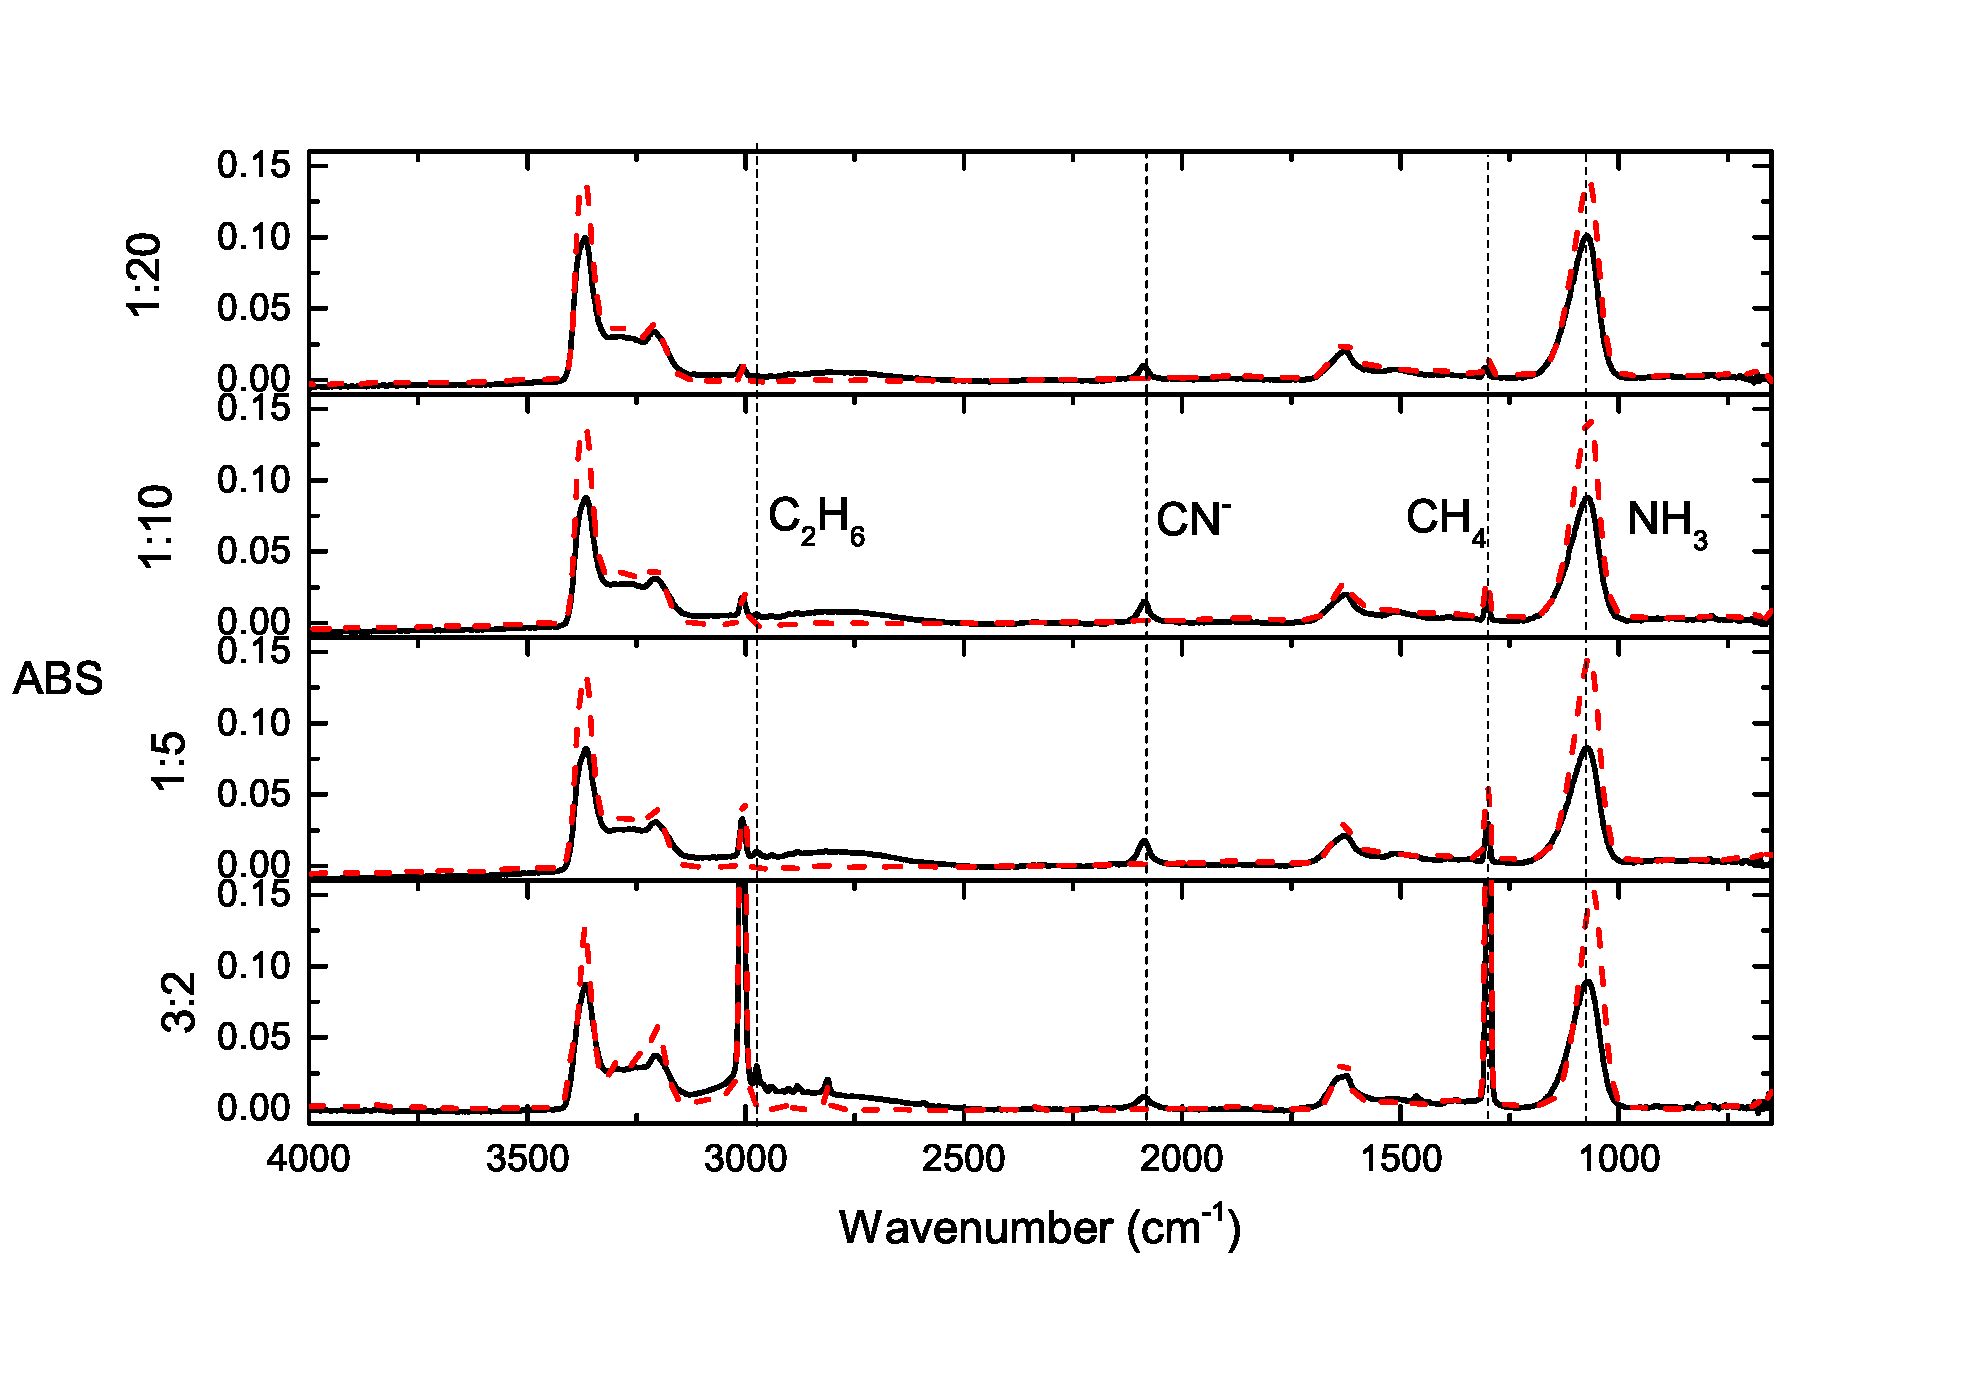
\includegraphics[width=\textwidth]{figures/chapter3/widerange.eps}
\caption{The the infra-red spectrum of CH$_4$ + NH$_3$ ice mixtures before irradiation (dashed) and VUV irradiated ice mixtures provided by MDHL. }
\label{fig:widerange}
\end{figure}

\begin{table}[htbp]
\caption{The peak positions of identified substances after irradiation in different configurations of ice mixtures.}
\label{tab:WavenumberMDHL}
\begin{tabular}{ccccccc}
\hline
\hline
\multicolumn{2}{c}{Literture assignments} & \multicolumn{4}{c}{CH$_4$+NH$_3$ ratio (MDHL)} &  \\
\hline
Wavenumber & Carrier  & 1:5  & 1:10  & 1:20  & 3:2  & Ref. \\
(cm$^{-1}$) &   & (cm$^{-1}$) & (cm$^{-1}$) & (cm$^{-1}$) & (cm$^{-1}$) &\\
\hline
3375 & $\nu_3$ (NH$_3$) & 3366 & 3366 & 3369 & 3367 & 1 \\
3290 & $2\nu_4$ (NH$_3$) & - & - & - & - & 1 \\
3210 & $\nu_1$ (NH$_3$) & 3207 & 3208 & 3210 & 3205 & 1 \\
3011 & $\nu_3$ (CH$_4$) & - & - & - & - & 2 \\
2972 & $\nu_{10}$ (C$_2$H$_6$) & 2975 & - & - & 2975 & 3 \\
2960 & C$_3$H$_8$ & - & - & - & 2960 & 7 \\
2941 & $\nu_8+\nu_11$ (C$_2$H$_6$) & 2940 & - & - & 2940 & 3 \\
2904 & $\nu_1$ (CH$_4$) & 2901 & - & - & 2901 & 5 \\
2879 & $\nu_5$ (C$_2$H$_6$) & 2882 & 2883 & - & 2882 & 3 \\
2814 & $\nu_2+\nu_4$ (CH$_4$) & - & - & - & 2815 & 5 \\
2083 & $\nu$ (CN$^-$) & 2088 & 2087 & 2088 & 2088 & 2 \\
1625 & $\nu_4$ (NH$_3$) & 1625 & 1625 & 1626 & 1631 & 1 \\
1514 & $\delta$ (NH$_2$) & 1509 & 1507 & 1505 & 1511 & 6 \\
1465-1440 & deform CH$_2$ scissor & 1461 & - & - & 1463 & 3,4 \\
1390-1370 & CH$_3$ sym deform & 1394 & 1394 & 1394 & 1372 & 4 \\
1298 & $\nu_4$ (CH$_4$) & 1301 & 1302 & 1305 & 1299 & 2 \\
1075 & $\nu_2$ (NH$_3$) & 1073 & 1072 & 1072 & 1072 & 1 \\
820 & $\nu_12$ (C$_2$H$_6$) & - & - & - & 820 & 3 \\
\hline
\end{tabular}\\
Reference: 1. Bossa et al. 2008 \cite{bossa2008carbamic} 2. Moore and Hudson 2003 \cite{moore2003infrared} 3. Kim et al. 2010 \cite{kim2010abiotic} 4. Socrates 2001 \cite{socrates2001infrared} 5. Bennet and Kaiser 2007 \cite{bennett2007formation} 6. Zheng et al. 2008 \cite{zheng2008formation} 7. Hudson and Moore 2004 \cite{hudson2004reactions}
\end{table}



To calculate the column density, we integrate the area under graph and divided by the absorption strength presented in table 3.2. We aware that there is an average error in absorption strengths of no more than 10 \%  when the pure ice is diluted in N$_2$ and H$_2$O \cite{richey2012near}. In our case, absorption strengths changes after CH$_4$ and NH$_3$ are mixed. For example, according to d' Hendecourt and Allamandola \cite{d1986time}, the band of NH$_3$ located at 1070 cm$^{-1}$ would not change much (from $1.1 \times 10^{-17}$ to $1.2 \times 10^{-17}$) when excess water is added to pure NH$_3$. For the case of CN$^-$, we know that CN$^-$ has a bond order =3 from its molecular orbitals. CN$^-$ which is different from CN (bond order 2.5).  CN stretching is very sensitive to the matrix environment. It can change by factor of 2 in amino acetonitrile and H$_2$O (1:3) \cite{borget2012aminoacetonitrile}. However, CN is not inspected in this chapter. Therefore, we are justified to use the same absorption strength throughout our discussion to estimate the column density of each species and how the absorption area changes with concentration ratios of ice mixtures and photon energy. Here, we adopt the absorption strengths stated in Table \ref{tab:Absorbance} \\

\begin{table}[htbp]
\caption{The strength of absorbance adopted in this thesis measured in literatures of pure ice samples}
\label{tab:Absorbance}
\begin{tabular}{cccccc}
\hline
\hline
Wavenumber (cm$^{-1}$) & Assignment  & Vibration & FWHM & A value ($\times 10^{-17}$) & Reference \\
\hline
2976 &  C$_2$H$_6$ & -CH$_3$ & - & 1.05 & 2 \\
2960 & C$_3$H$_8$ & -CH$_2$- & - & 2.58 & 2 \\
2086 & CN$^-$ & CN & - & 1.8 & 3 \\
1297 & CH$_4$ & CH deformation & 8 & 0.61 & 1 \\
1070 & NH$_3$ & "umbrella mode" & 68 & 1.7 & 1 \\
\hline
\end{tabular}
Reference: 1. d'Hendecourt and Allamandola (1986)\cite{d1986time} 2. Moore and Hudson (1998)\cite{moore1998infrared} 3. Noble et al. (2013) \cite{noble2012thermal}
\end{table}


\section{Reaction mechanisms} %mechanisms

\subsection{C$_2$H$_6$}

\begin{figure}
\centering
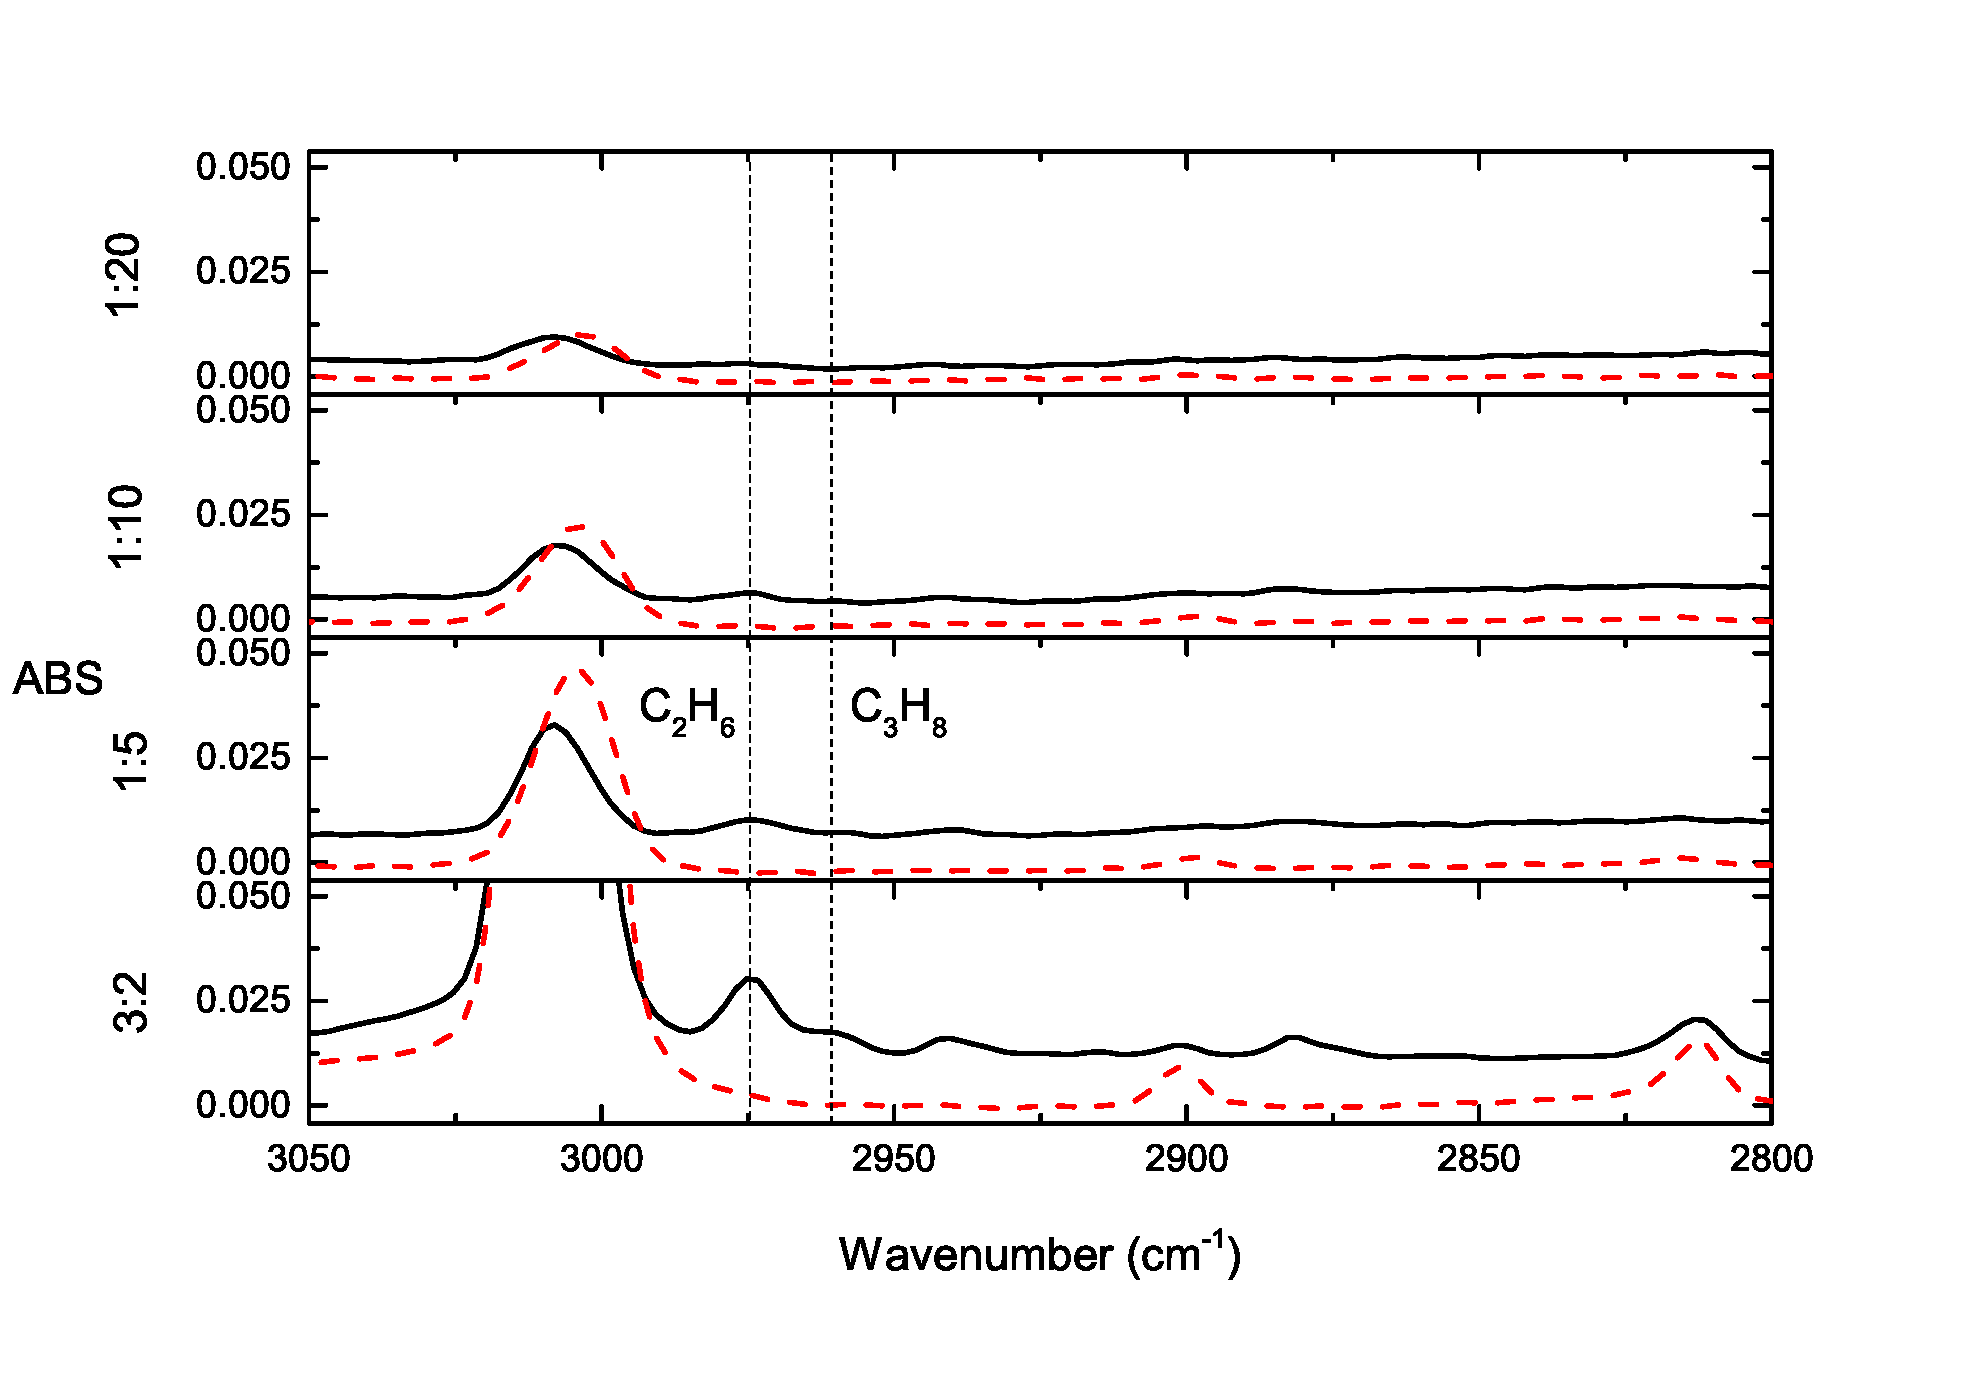
\includegraphics[width=\textwidth]{figures/chapter3/C2H6.eps}
\caption{The the infra-red spectrum of CH$_4$ + NH$_3$ ice mixtures of C$_2$H$_6$ and C$_3$H$_8$ before irradiation (dashed) and VUV irradiated ice mixtures provided by MDHL. }
\label{fig:C2H6}
\end{figure}

The assignment of C$_2$H$_6$ is confirmed by several bands listed in table \ref{tab:WavenumberMDHL}. Figure \ref{fig:C2H6} is a zoomed view of figure \ref{fig:widerange}. The absorption peak located at 2075 cm$^{-1}$ corresponds to the strongest vibration of C$_2$H$_6$. The formation of C$_2$H$_6$ in astrophysical environment is mainly through a combination with 2 CH$_3$ radicals  \cite{bennett2006laboratory}:

\begin{equation}
CH_4 + hv \rightarrow CH_3
\label{eq:CH3}
\end{equation}
\begin{equation}
2 CH_3 \rightarrow C_2H_6
\label{eq:C2H6}
\end{equation}

The energy required to produce 1 CH$_3$ radical from CH$_4$ is 4.42 eV.  Recombination of 2 CH$_3$ radicals to form C$_2$H$_6$ releases 3.74 eV. The process in \ref{eq:C2H6} is a no-barrier exothermic process. Note that C$_2$H$_6$ is not detected in CH$_4$ to NH$_3$=1:20 ice mixtures. Figure \ref{fig:lab_C2H6} shows the temporal formation column density of C$_2$H$_6$ in different configurations of irradiated ice mixtures.  As the formation only depends on CH$_4$, we may use first order kinetics equation to fit the column density versus photon dose.

\begin{equation}
[A] = [A]_0(1 - e^{-k_1 t})
\label{eq:1step}
\end{equation}
The fitting results are shown in table \ref{tab:fittingC2H6}.

\begin{figure}
\centering
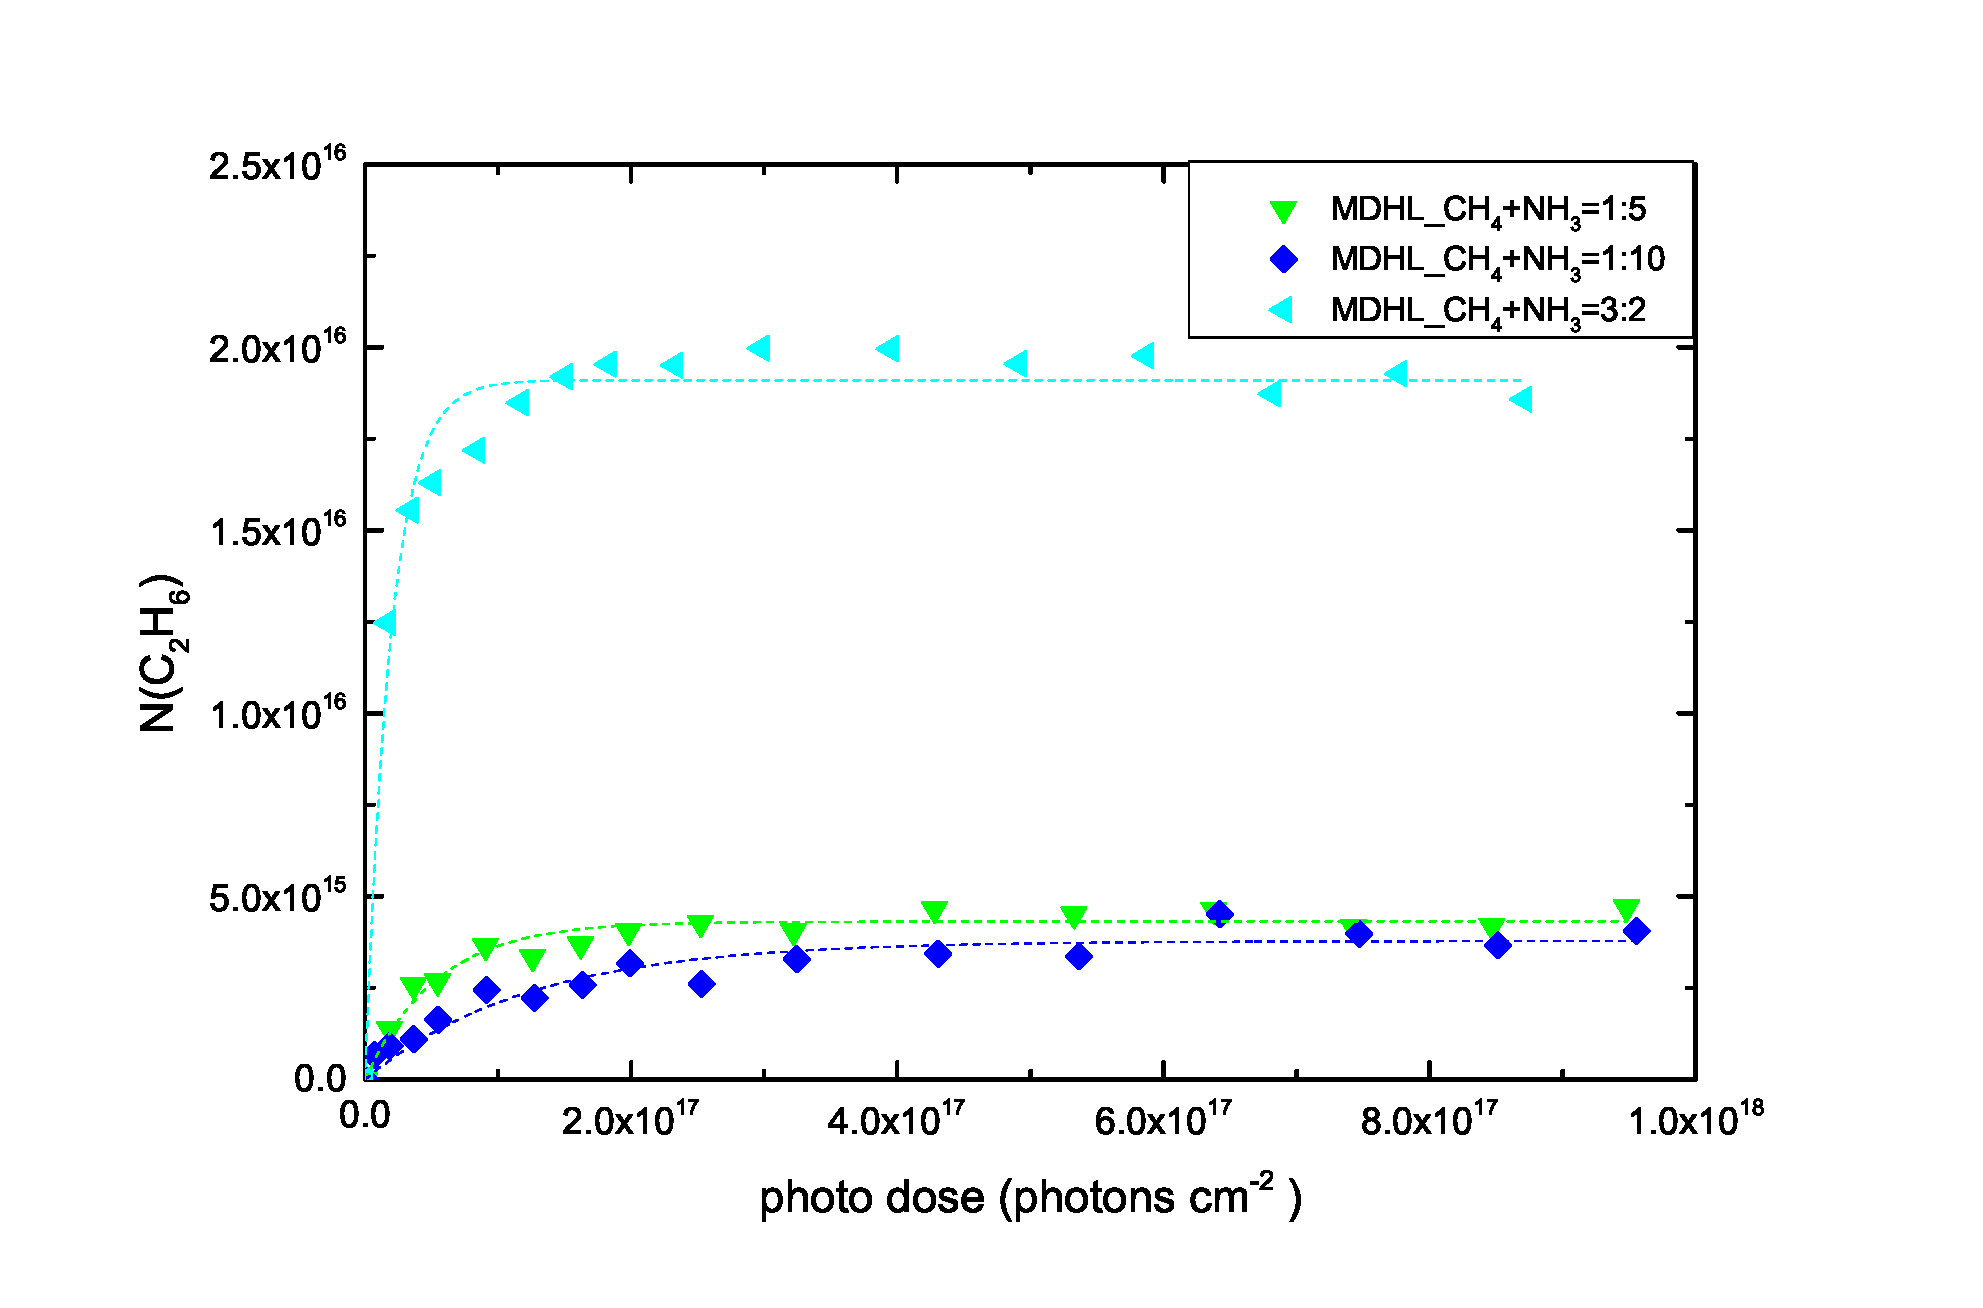
\includegraphics[width=\textwidth]{figures/chapter3/Lab_C2H6.eps}
\caption{The column density of C2H6 during CH4 + NH3 ice mixtures irradiated by MDHL. }
\label{fig:lab_C2H6}
\end{figure}

\begin{table}[htbp]
\caption{The fitting results of C$_2$H$_6$ by [C$_2$H$_6$]=[C$_2$H$_6$]$(1 - e^{-k_1 t})$}
\label{tab:fittingC2H6}
\begin{tabular}{ccc}
\hline
\hline
Ratio of CH$_4$+NH$_3$ & A (x10$^{15}$ molecules cm$^{-2}$) & k (x10$^{-17}$ photon$^{-1}$) \\
\hline
1:10 & 2.90 $\pm$ 1.25 & 0.92 $\pm$ 0.15 \\
1:5 & 4.16 $\pm$ 0.28 & 2.28 $\pm$ 0.28 \\
3:2 & 19.2 $\pm$ 0.15 & 5.28 $\pm$ 0.25 \\
\hline
\end{tabular}
\end{table}

From table \ref{tab:fittingC2H6}, the production rate is nearly proportional to the initial CH$_4$ concentration.


\subsection{C$_3$H$_8$}

The peak positioned at 2960 cm$^{-1}$ belongs to –CH$_2$- so we assigned that as C$_3$H$_8$, as the shortest carbon chain. The signal to noise ratio in CH$_4$+NH$_3$ = 1:10 is poor that we can not quantize the amount of C$_3$H$_8$ (figure \ref{fig:C2H6}).

It is a secondary product formed by a combination of either C$_2$H$_6$ + CH$_2$ (equation \ref{eq:C3H81})or C$_2$H$_4$ + CH$_4$ (equation \ref{eq:C3H82}).
\begin{equation}
C_2H_6 + CH_2 \rightarrow C_3H_8
\label{eq:C3H81}
\end{equation}
\begin{equation}
C_2H_4 + CH_4 \rightarrow C_3H_8
\label{eq:C3H82}
\end{equation}

By modern peak fitting method, we deconvoluted the overlapped C$_2$H$_6$ and C$_3$H$_8$ into two gaussians.

\subsection{CN$^-$}

\begin{figure}
\centering
\includegraphics[width=\textwidth]{figures/chapter3/CN.eps}
\caption{The infra-red spectrum of CH$_4$ + NH$_3$ ice mixtures of C$_2$H$_6$ and C$_3$H$_8$ before irradiation (dashed) and VUV irradiated ice mixtures provided by MDHL. }
\label{fig:CN}
\end{figure}

From infra-red absorption spectrum (figure \ref{fig:CN}) and their positions, we assigned the peak 2086 cm$^{-1}$ to CN$^-$  but not a combination of HCN and CN$^-$. The assignment is based on a absence in CN bending mode at 848 cm$^{-1}$. In the case CH$_4$ + NH$_3$ = 3:2, we may observe a peak located at 820 cm$^{-1}$, which is with a FWHM half of HCN and it is eliminated at 50 K during the warm-up phase. Since 50 K is the desorbing temperature of C$_2$H$_6$ and the peak position is the close to v12 mode of C$_2$H$_6$, we believe that the 820 cm$^{-1}$ peak is contributed by C$_2$H$_6$. Therefore, we may assign our peak located at 2086 cm$^{-1}$ as purely CN$^-$.\\

\begin{figure}
\centering
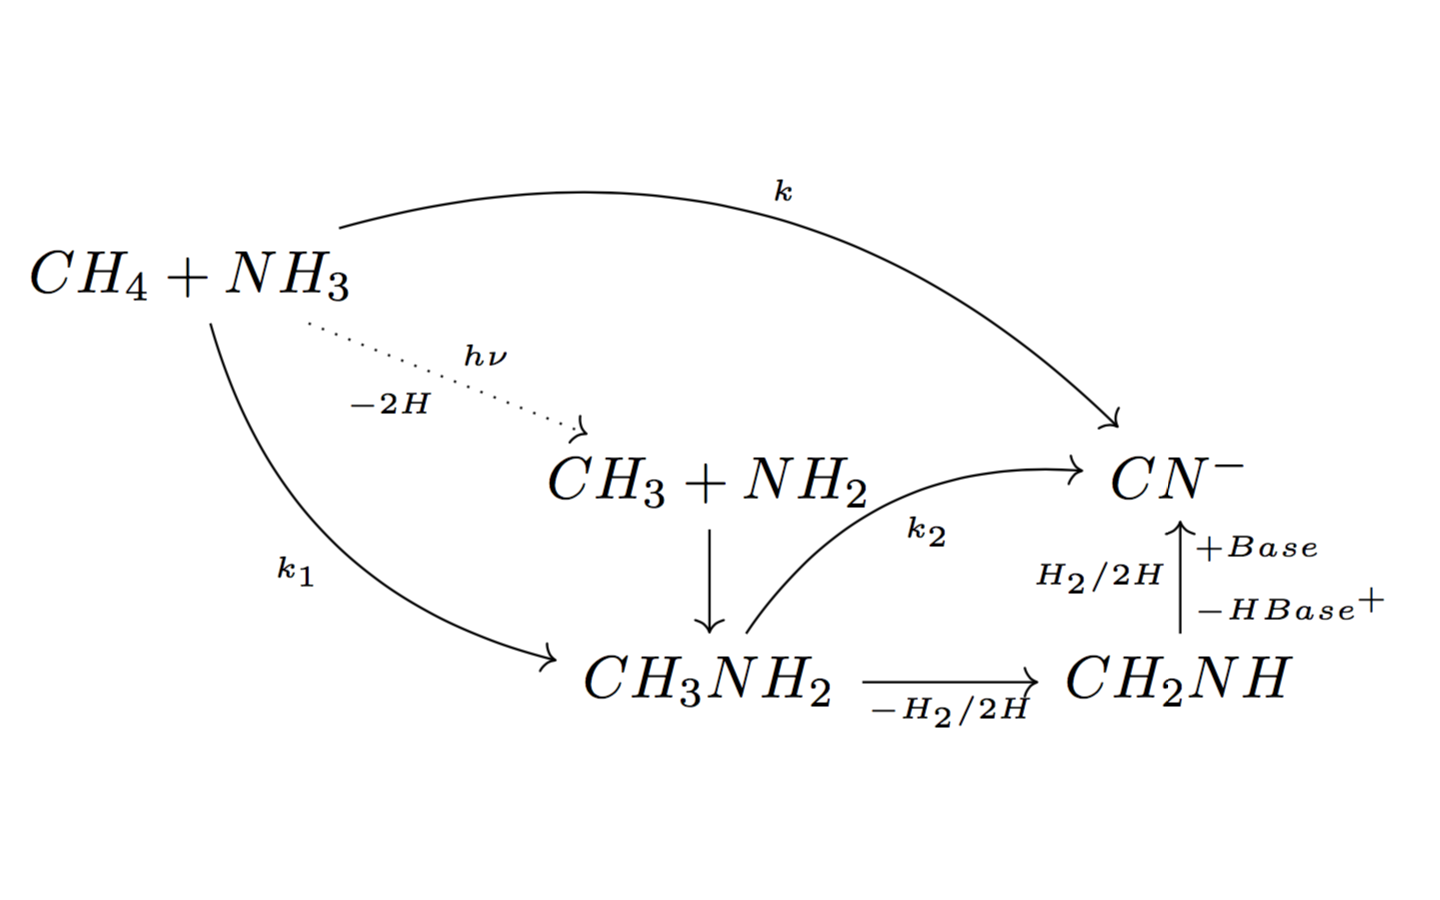
\includegraphics[width=\textwidth]{figures/chapter3/CNmechanism}
\caption{The formation mechanism of CN$^-$ proposed by Kim and Kaiser(2011). }
\label{fig:CNmechanism}
\end{figure}

The formation mechanism of CN$^-$ at low temperature was first suggested by Kim and Kaiser \cite{kim} to be two step reaction mechanism with methylamine as intermediate. CH$_4$ and NH$_3$ irradiated by photon to become CH$_3$ and NH$_2$ radical (figure \ref{fig:CNmechanism}, followed by propagation and recombination of radicals becoming CH$_3$NH$_2$ and dehydrogenation and acid-base reaction to form CN$^-$.
Although Kim and Kaiser \cite{kim} used 1.5 keV electron as energy source to simulate the cosmic ray induced photochemistry, this formation mechanism also applies in our photon irradiation experiments because we can also detect the methylamine during our warm-up phase. The ion fragment with m/z=31 is assigned as CH$_3$NH$_2$$^+$ and detectable in all ratios of our CH$_4$+NH$_3$ experiments (figure \ref{Mass31}).

\begin{figure}
\centering
\includegraphics[width=\textwidth]{figures/chapter3/Mass31.eps}
\caption{The m/z=31 detected by QMS during warm-up with heating rate 1 K/min in different configurations of ice mixtures.}
\label{Mass31}
\end{figure}

By the deviation performed in section \ref{sec:Reaction_Rate_Laws}, we have a rate equation for consecutive reactions \ref{eq:rate7}. With one of the reactant larger than another, we applied the pseudo first order assumption. With equation \ref{eq:rate7}, we fitted the formation of CN$^-$ (figure \ref{fig:CNrate})and found that one of the rate constant is always larger than the other in all of the ratios. The fitting results are averaged by more than two experiments and are shown in table \ref{tab:CNrate}.The results of Kim and Kaiser is also listed into the table, they could observe a two-step reaction mechanism in production of CN$^-$ in CH$_4$+NH$_3$ (3:1) experiments with electron current 0.1 $\mu$A. However, when they increased the electron flux to 1 $\mu$A for irradiation C$_n$H$_{2n+2 (n=1-6)}$ and NH$_3$ ice mixtures, they also observed a one-step reaction mechanism.

\begin{figure}
\centering
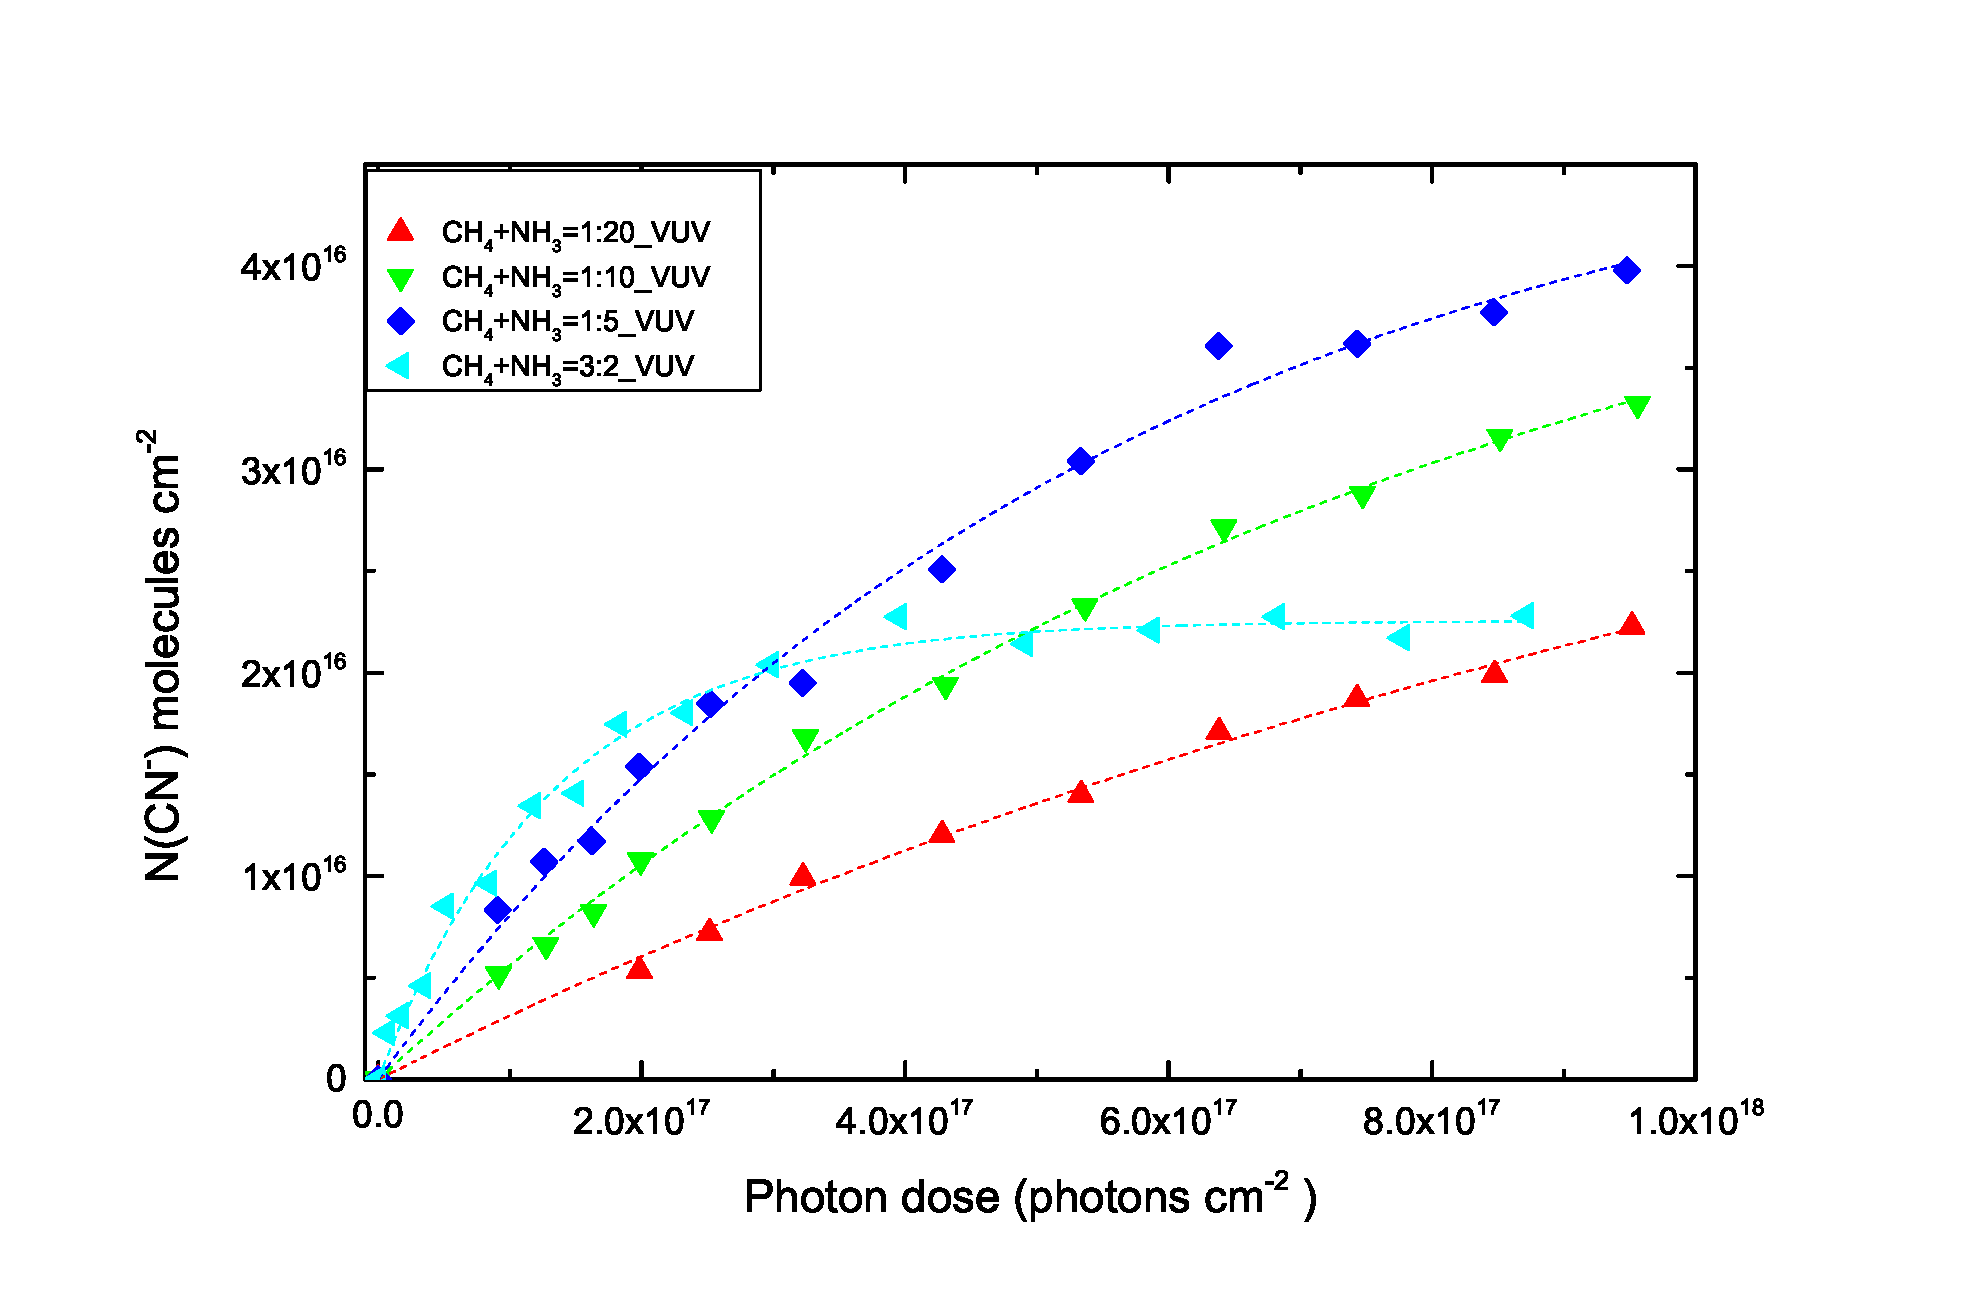
\includegraphics[width=\textwidth]{figures/chapter3/Overall_CN_rate.eps}
\caption{The column density of CN$^-$ accumulated when different configurations of CH$_4$ + NH$_3$ ice mixtures are irradiated by VUV photons provided by MDHL. The dotted lines are fits of column densities by equation \ref{eq:rate7}.}
\label{fig:CNrate}
\end{figure}

\begin{table}[htbp]
\caption{The fitting results of CN$^-$ by equation \ref{eq:rate7}}
\label{tab:CNrate}
\begin{tabular}{cccc}
\hline
\hline
Ratio of CH$_4$+NH$_3$ & A (x10$^{16}$ molecules cm$^{-2}$) & k$_1$ (x10$^{-18}$ photon$^{-1}$) & k$_2$ (photon$^{-1}$)\\
\hline
1:20 & 4.75 $\pm$ 0.40 & 0.70 $\pm$ 0.09 & >1 \\
1:10 & 4.51 $\pm$ 0.18 & 1.33 $\pm$ 0.13 & >1 \\
1:5 & 4.61 $\pm$ 0.18 & 1.93 $\pm$ 0.19 & >1 \\
3:2 & 2.24 $\pm$ 0.03 & 8.21 $\pm$ 0.70 & >1 \\
\hline
\end{tabular}\\
A represents the amount of CN$^-$ we may obtain when irradiated the ice for infinitely long.\
\end{table}

\section{The Concentration Effect in formation of Cyanide ions and Ethane}

\subsection{Cyanide ion}

From table \ref{tab:CNrate}, we may observe that the rate k$_1$ is nearly proportional to the concentration of CH$_4$.  As CH$_4$ to NH$_3$ ratio increases, more CH$_4$ are involved in CH$_3$ radical formation, thus there are more CH$_3$ radicals to produce CH$_3$NH$_2$ intermediates.

In CH$_4$ to NH$_3$ =3:2 ice mixtures, A is about half of that of the other ratios. The reduction is mainly because NH$_2$ (forming CH$_3$NH$_2$) has a competing relationship with CH$_2$, CH$_3$ and C$_2$H$_4$ radicals (forming C$_2$H$_6$ and C$_3$H$_8$). This competition supresses the production of intermediate CH$_3$NH$_2$, thus the formation of CN$^-$. Therefore, the yield of CN$^-$ is the least in CH$_4$ to NH$_3$ ice mixture with ratio 3:2 while the yield of C$_2$H$_6$ is the greatest in the mixture with the same ratio(table \ref{tab:CNrate}), (table \ref{tab:fittingC2H6})\\

Considering the normalized CN$^-$ with respect to the initial CH$_4$(figure \ref{fig:CN_CH4}), the formation of CN$^-$ is more efficient in low CH$_4$ concentration ice mixtures. At low CH$_4$ concentration, there are excess NH$_3$ which can aggregate mobile CH$_3$ radicals, preventing meeting another CH$_3$ radical or C$_2$H$_4$. Therefore the production of C$_2$H$_6$ is greatly suppressed and more CN$^-$ will be produced.

\begin{figure}
\centering
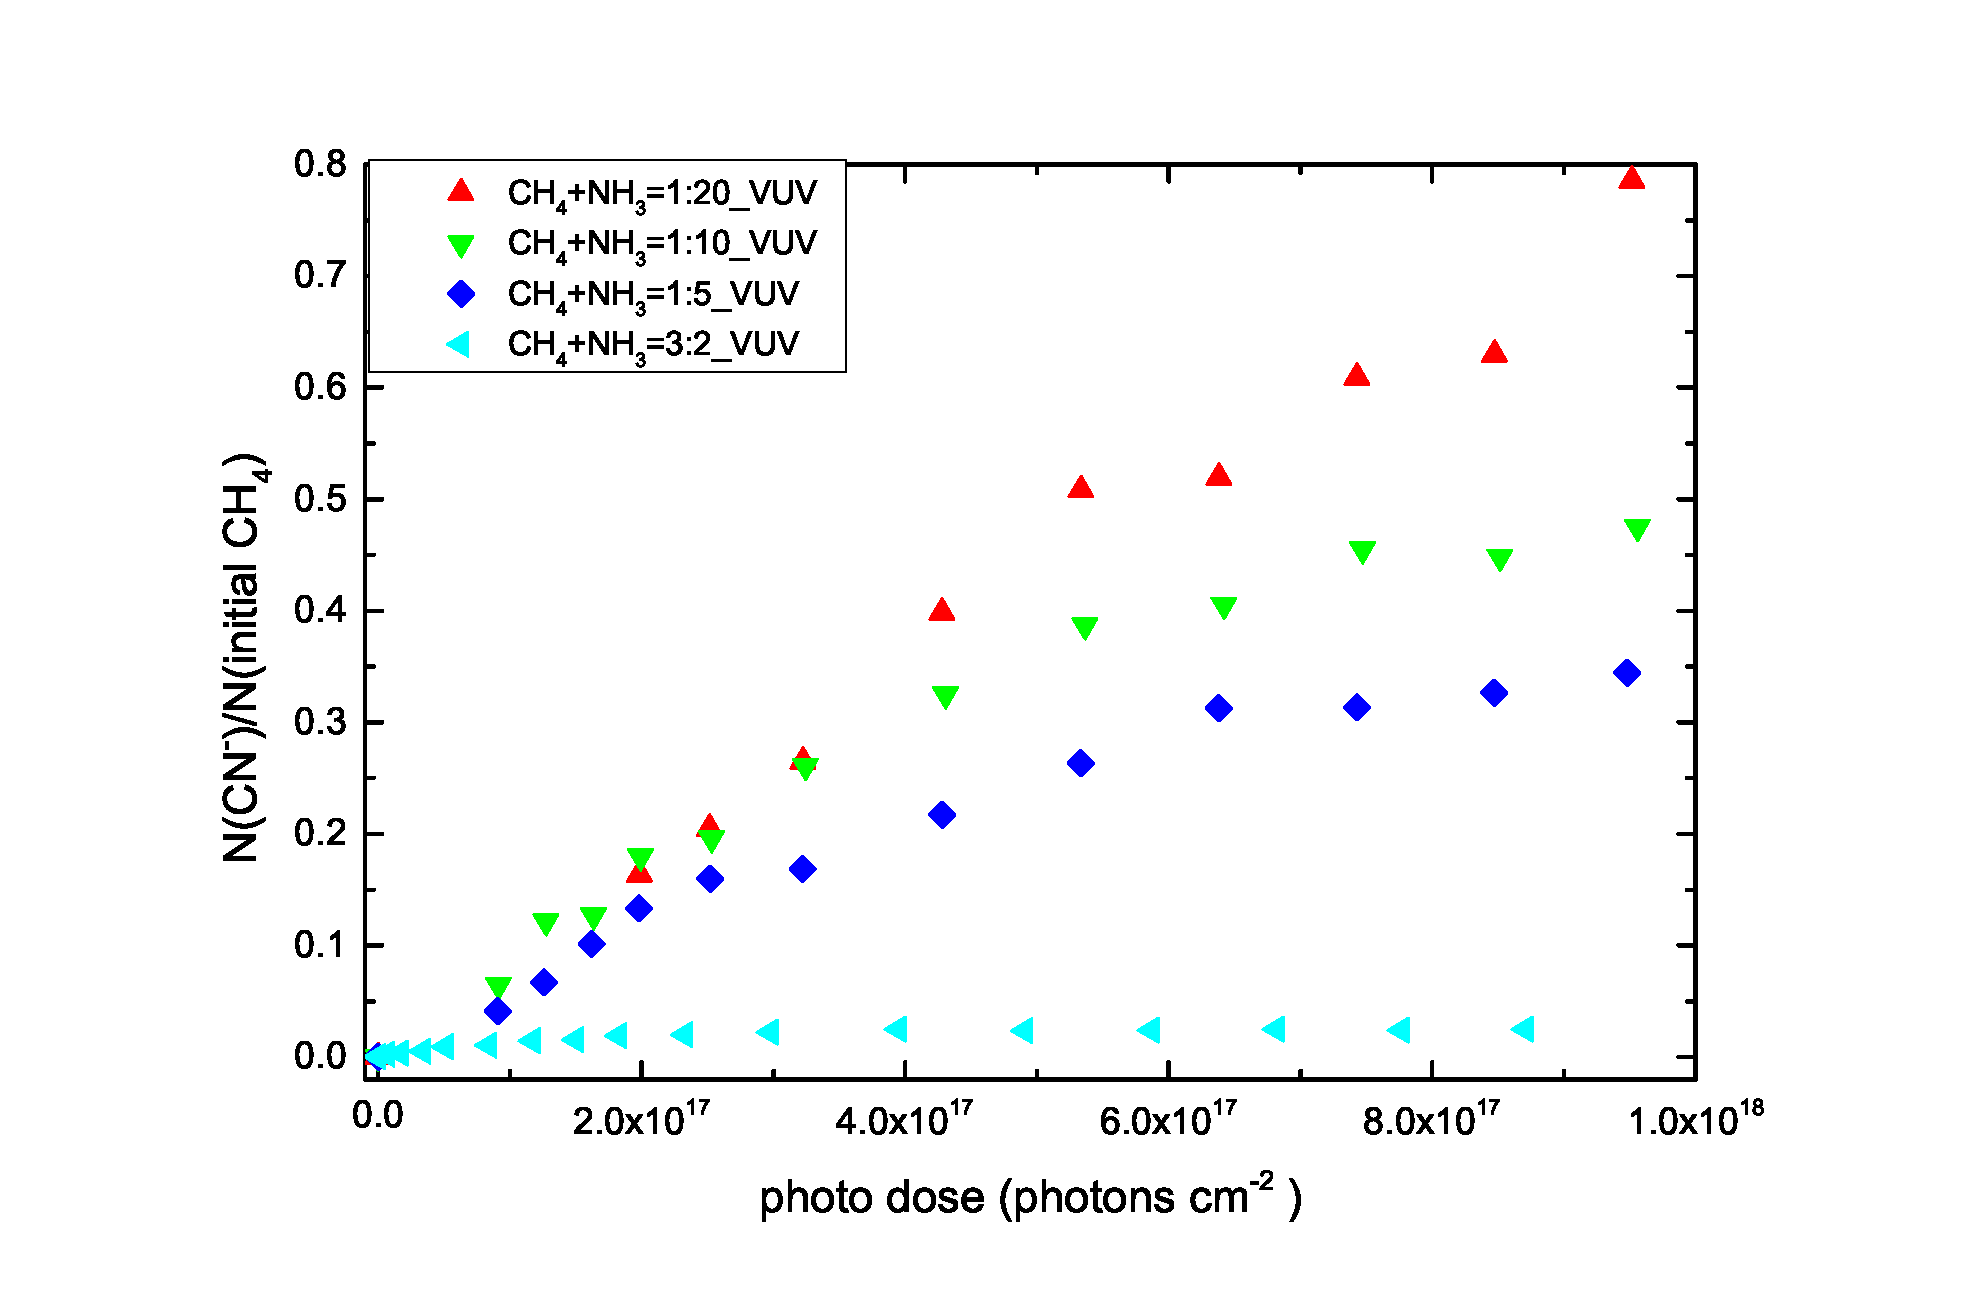
\includegraphics[width=\textwidth]{figures/chapter3/CN_CH4.eps}
\caption{The column density of CN$^-$ divided by initial CH$_4$ accumulated when different configurations of CH$_4$ + NH$_3$ ice mixtures are irradiated by VUV photons provided by MDHL.}
\label{fig:CN_CH4}
\end{figure}

\subsection{Ethane}


\begin{figure}
\centering
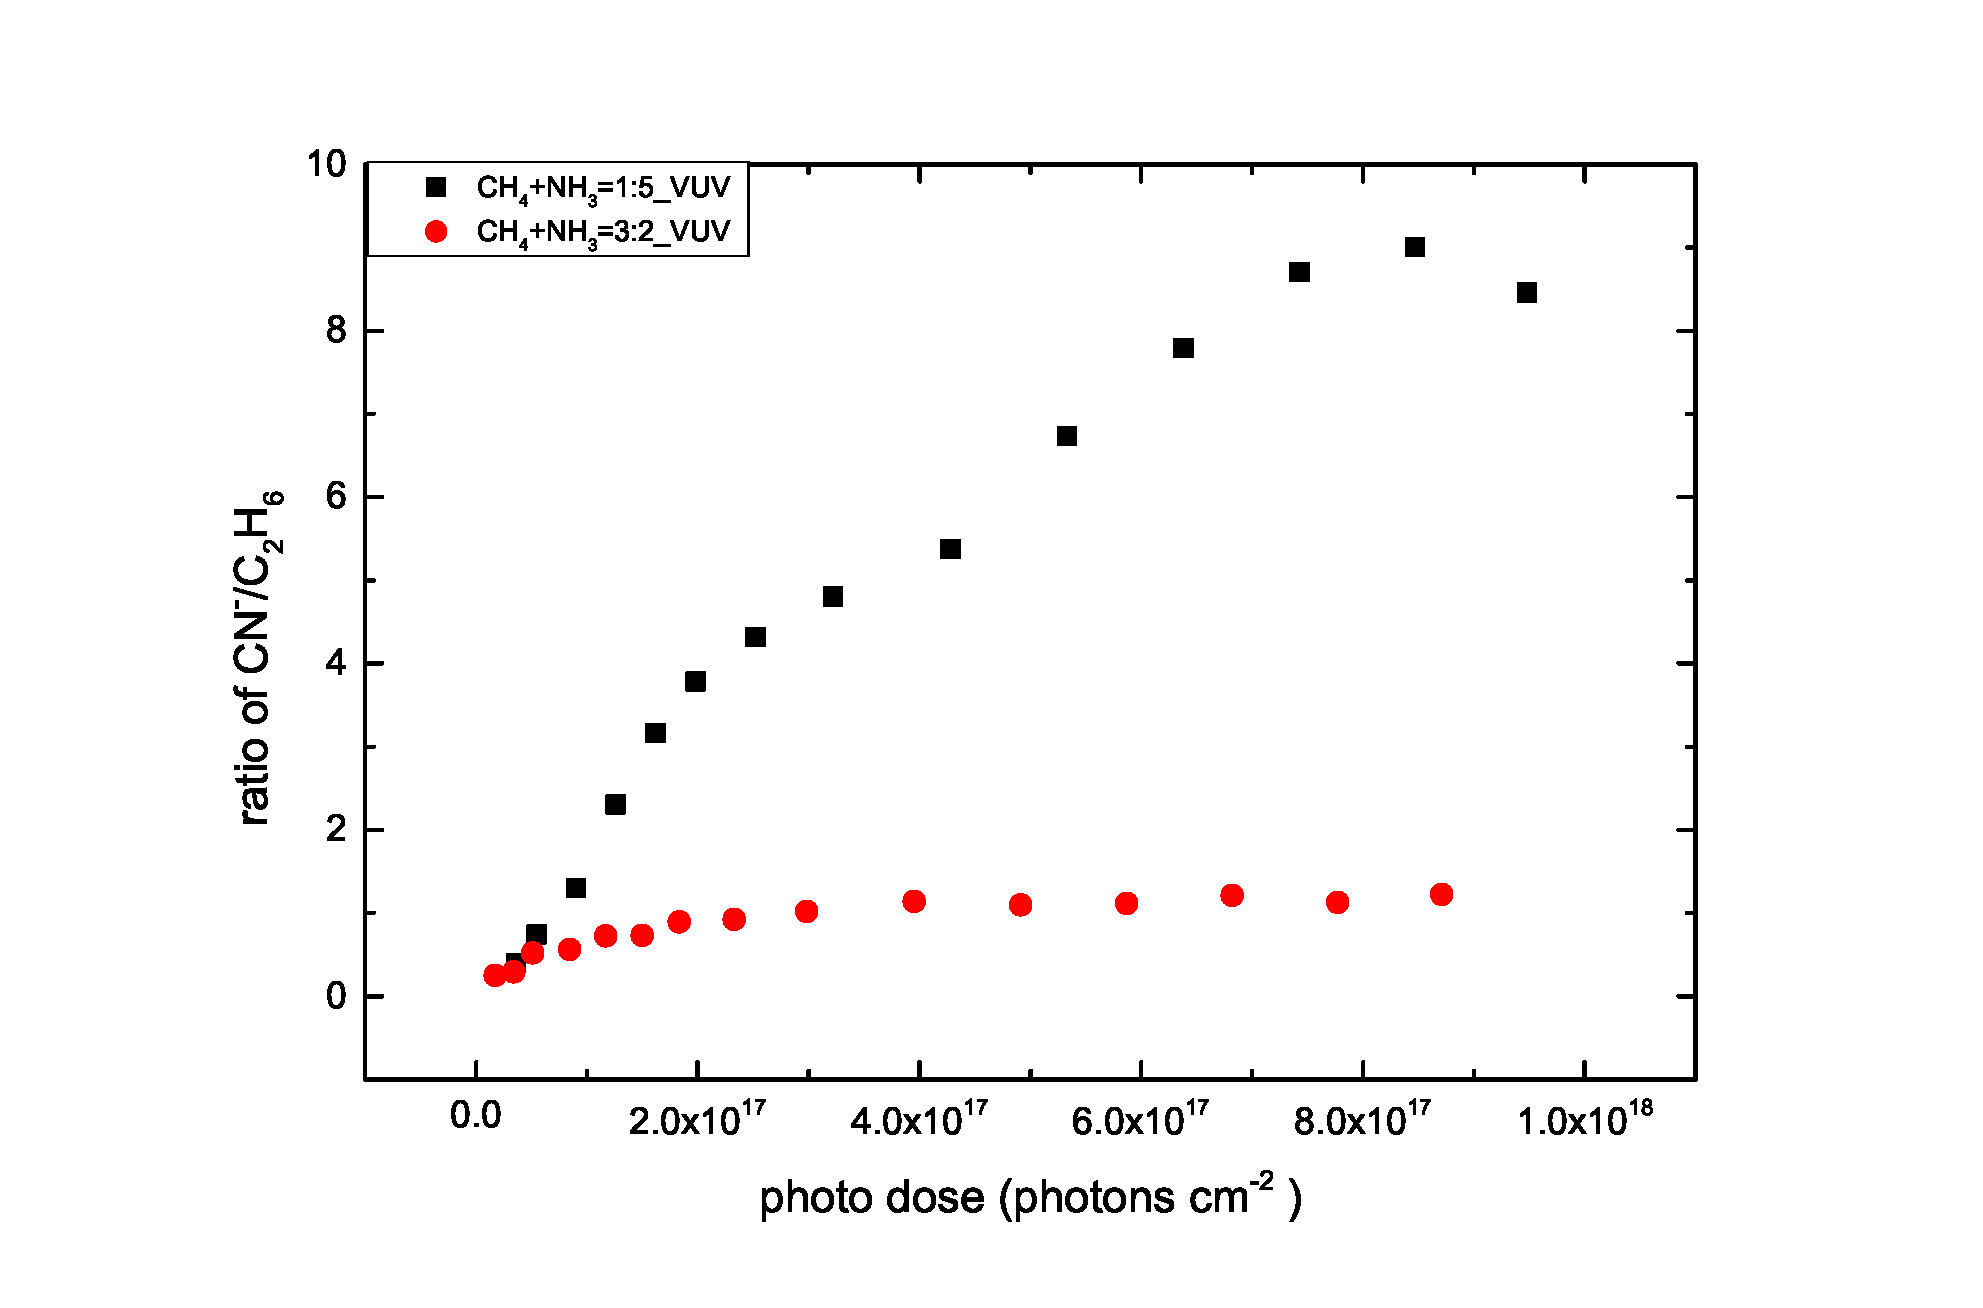
\includegraphics[width=\textwidth]{figures/chapter3/CN_C2H6.eps}
\caption{The column density of CN$^-$ divided by C$_2$H$_6$ accumulated when different configurations of CH$_4$ + NH$_3$ ice mixtures are irradiated by VUV photons provided by MDHL.}
\label{fig:C2H6_CN}
\end{figure}

Considering the case of ratio of CN$^-$ divided by C$_2$H$_6$,the formation of CN$^-$ in ice mixtures with diluted CH$_4$ has more CN$^-$ formed then C$_2$H$_6$. It is because ice mixtures with with higher concentrations in CH$_4$ is more effective for one CH$_3$ radical to combine with another CH$_3$ radical. On the contrast, CH$_3$ radicals formed in the ice mixtures with diluted CH$_4$ concentrations are aggregated by NH$_3$. Therefore, CN$^-$ is less efficient to form in ice mixtures with excess NH$_3$.

\subsection{Propane}

\begin{figure}
\centering
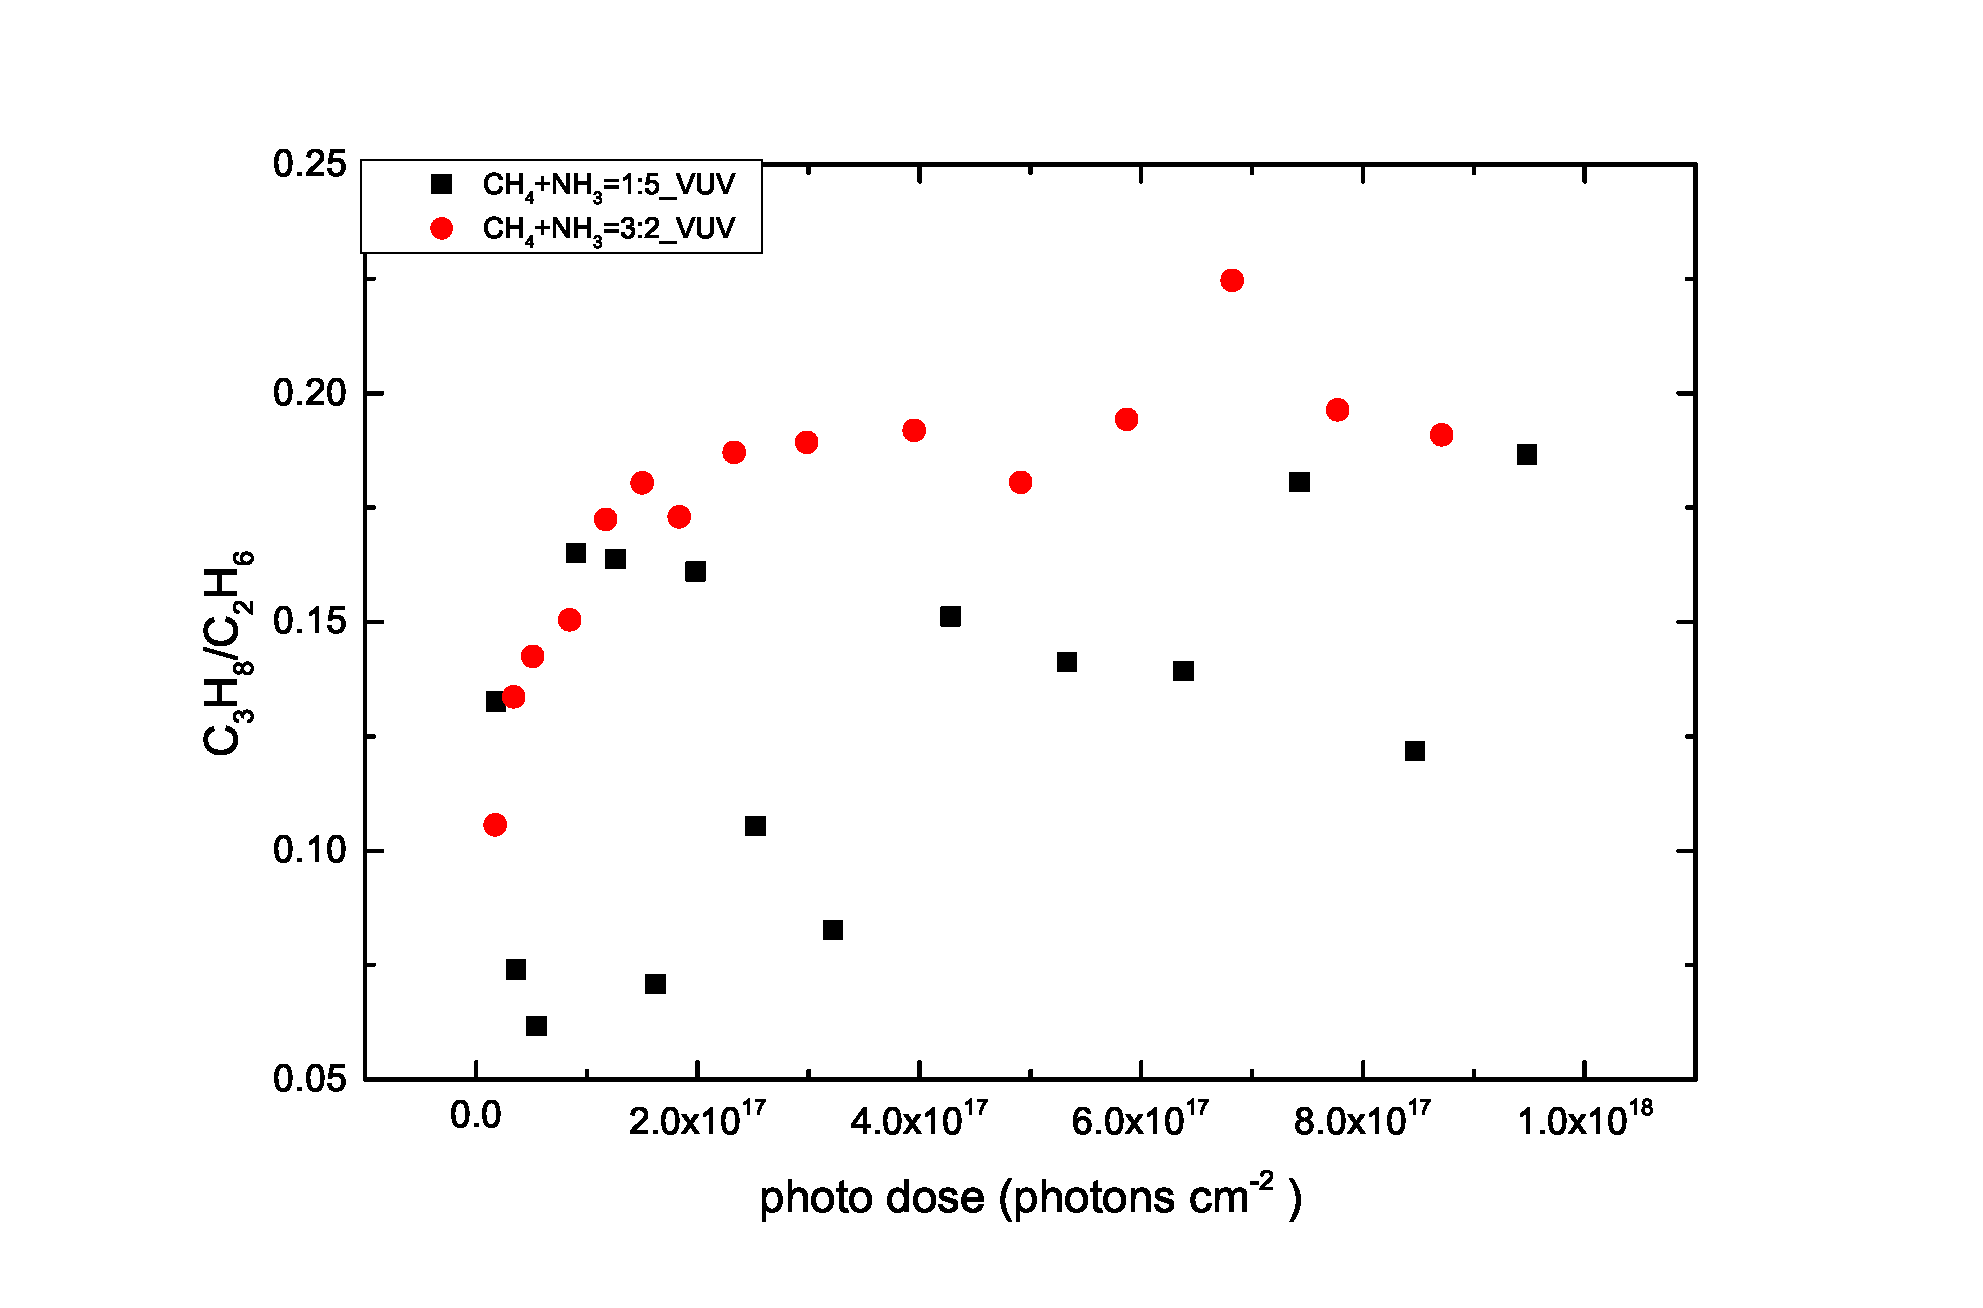
\includegraphics[width=\textwidth]{figures/chapter3/Lab_C3H8_C2H6.eps}
\caption{The column density of C$_3$H$_8$ divided by C$_2$H$_6$ accumulated when different configurations of CH$_4$ + NH$_3$ ice mixtures are irradiated by VUV photons provided by MDHL.}
\label{fig:C2H6_C3H8}
\end{figure}

C$_3$H$_8$ forms based on to the C$_2$H$_6$ \ref{fig:C2H6_C3H8} is the plot with column densities of C$_2$H$_6$ divided by C$_3$H$_8$. We may see that the ratio in CH$_4$+NH$_3$ =1:5 experiment is around 6 where CH$_4$+NH$_3$ =3:2 is around 3. This shows that the amount of C$_3$H$_8$ in CH$_4$+NH$_3$ =3:2 experiment is higher. It is rather difficult for C$_3$H$_8$ to form in CH$_4$+NH$_3$ = 1:5 experiments because NH$_3$ aggregated them. The formation of C$_3$H$_8$ in CH4+NH3 =1:5 and 3:2 experiments has given a reasonable explanation about why C$_2$H$_6$ formation is most efficient in CH$_4$+NH$_3$ =1:10 experiments.



\section{Photon Energy Effect - EUV and VUV} %EUV & VUV

According to Blanksby and Ellison \cite{blanksby2003bond}, the dissociation energy for CH$_4$, becoming CH$_3$, CH$_2$ CH and C are 4.55, 4.79, 4.39 and 3.51 eV respectively at 298 K. Whereas dissociation energy for NH$_3$, becoming NH$_2$ is 4.67 eV at 298 K.

Considering our MDHL with average energy of 9.27 eV, all of the above fragments may exist either in the form of radicals or combined with other radicals to form heavier molecules in our ice mixtures. Although Increasing the photon energy does not create new fragmentation pathway, the choice of fragmentation pathways depends on photon energy.

Several gaseous state measurements also support this statement. First, Gans et al. (2011) \cite{gans2011photolysis} changed VUV photon wavelengths from 121.6 nm to 118.2 nm to dissociate the CH$_4$ molecules and ionize the fragments with the corresponding photon energy. Changing the output of the pulsed laser from 121.6 to 118.1 nm significantly changed the ratio of CH$_3^+$ and CH$_2^+$, produced from fragmentation, from 1: 1 to 1:2. This slight change of photon energy, from 10.2 eV to 10.4 eV has a significant change in the ratio between different pathways.

Second, an EUV fragmentation experiment done by Tsai et al. \cite{tsai1980mass} used 30.4 nm to photo-dissociate CH$_4$ and tested it by time�� - of ��- flight mass spectrometer yields CH$_3^+$: CH$_2^+$: CH$^+$: C$^+$ = 1 :0.32: 0.118: 0.0237 (Tsai 1980). Consider the ratios of CH$_3$ to CH$_2$ radicals, it is around 3 to 1, which is in contrast to the experiment results of Gans et al. (2011)\cite{gans2011photolysis}. Although both of them are gaseous state experimental results, it is uncertain that if increasing photon energy can produce more CH$_2$ radicals.

Thirdly, a group varies ratios of CH$_4$ + NH$_3$ mixtures and irradiate with far UV irradiation at 134 nm \cite{bossard1980far}. However, this group only used gas chromatography to analyse the final products and their reaction is carried in gas phase in room temperature. We aware that the VUV absorption spectra of CH$_4$ in solid phases is different from gaseous phases \cite{cruz2014vacuum}, so the exact photo dissociation fragmentation ratios by EUV nor VUV irradiations in astronomical environments are still unknown. It is worthwhile for us to perform the experiment by EUV irradiation to see if  EUV irradiation can generate any new products on the surface of Charon, or any difference in yield. Despite the photon energy of our MDHL is enough to dissociate both the CH$_4$ and NH$_3$ molecules, we further increase photon energy to He II 30.4 nm to examine the differences in photo-products. 

\begin{figure}
\centering
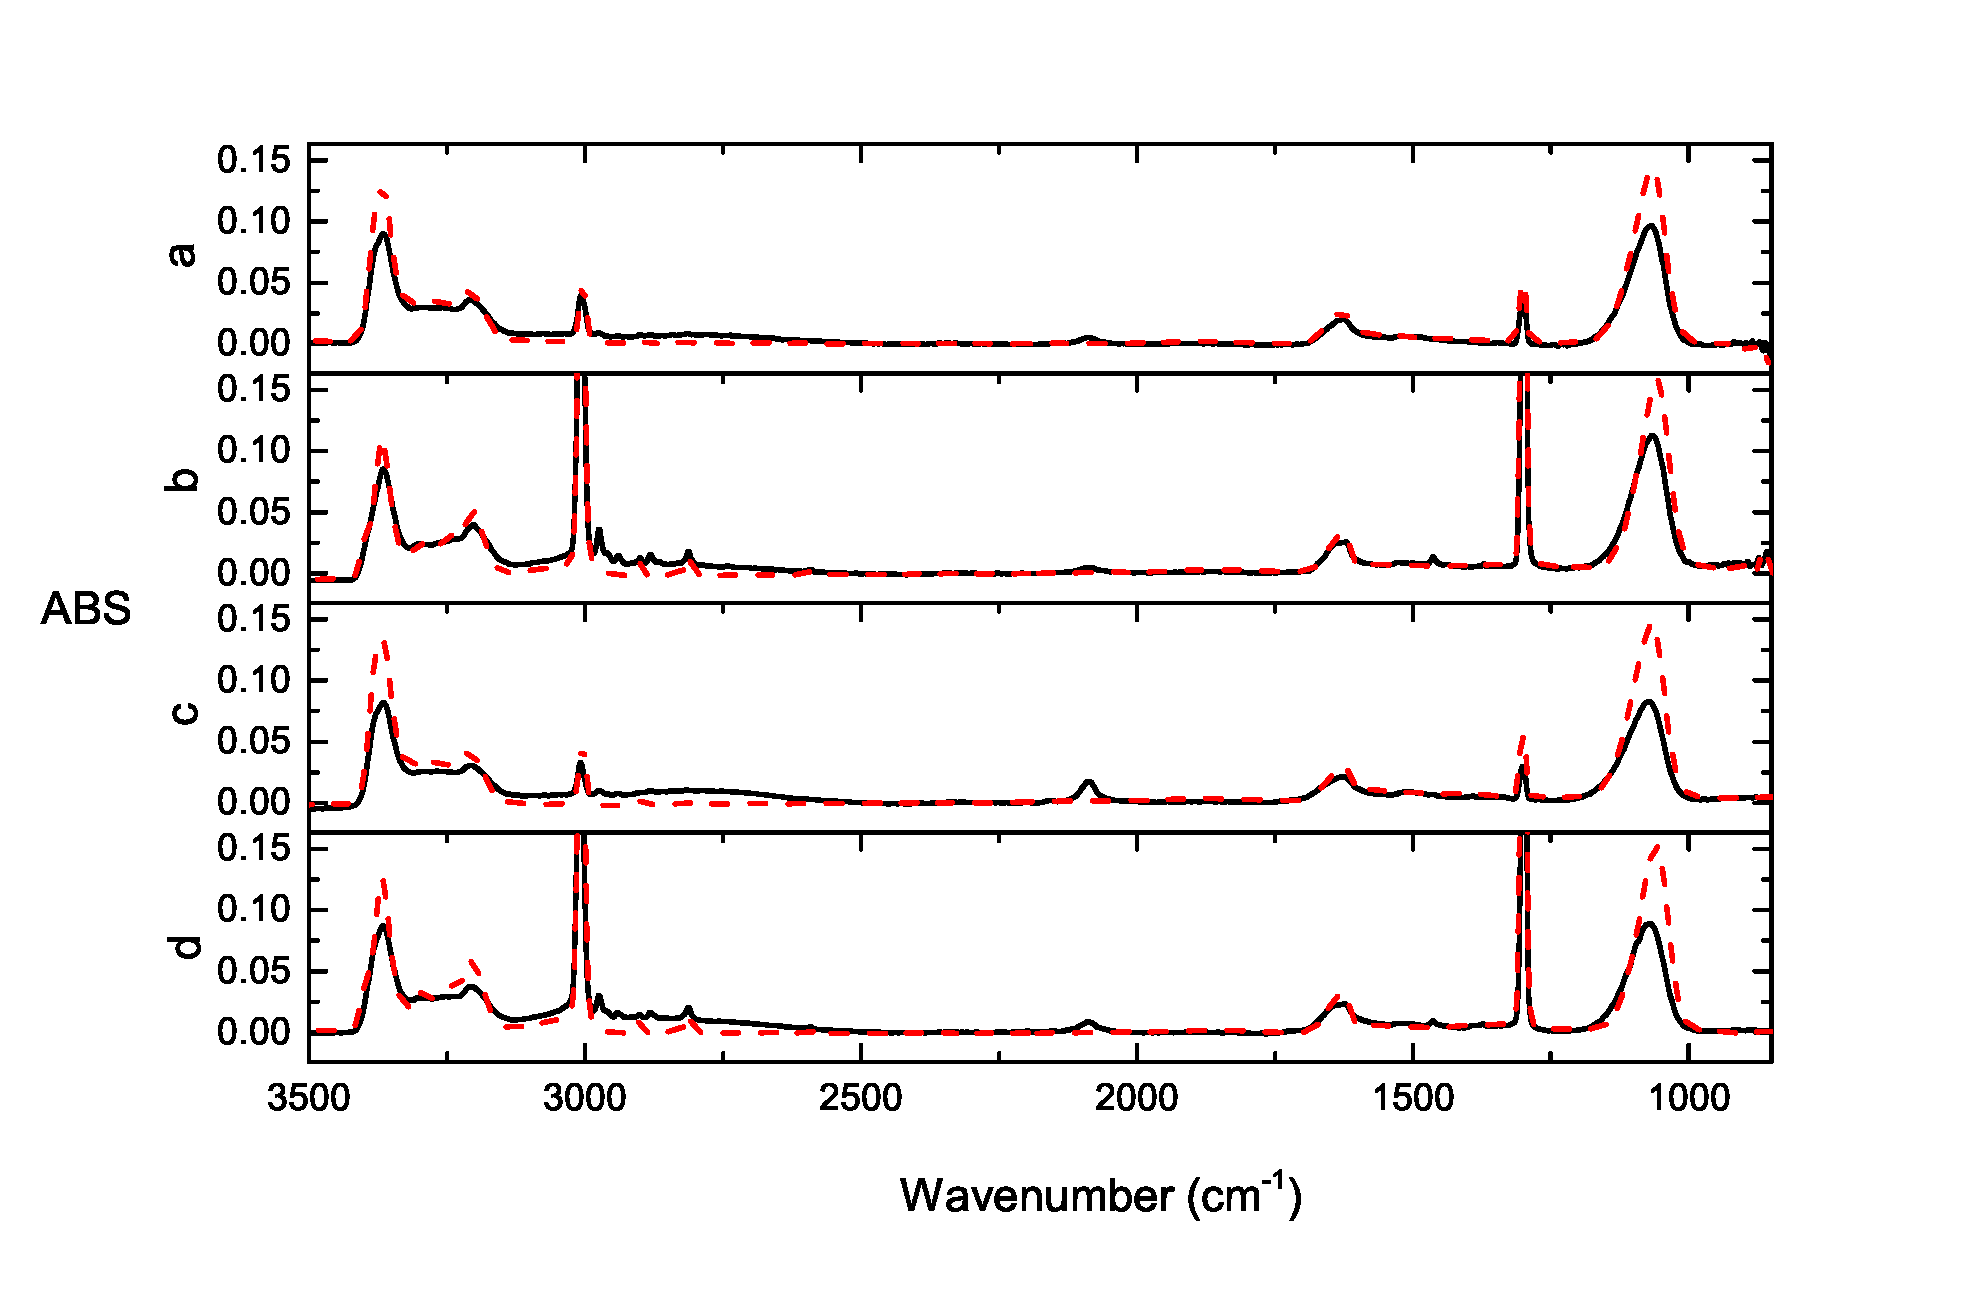
\includegraphics[width=\textwidth]{figures/chapter3/NSRRC_MDHL_IR.eps}
\caption{The the infra-red spectrum of CH$_4$ + NH$_3$ ice mixtures before irradiation (dashed) and VUV and EUV (solid) irradiated ice mixtures provided by MDHL. (a) and (b) are EUV irradiated CH$_4$+NH$_3$ = 1:5 and 3:2 ice mixtures respectively, and (c) and (d) are VUV irradiated CH$_4$+NH$_3$ = 1:5 and 3:2 ice mixtures respectively.}
\label{fig:NSRRC_MDHL_IR}
\end{figure}

Table \ref{tab:WavenumberNSRRC} shows the identified peaks of CH$_4$+NH$_3$ ice mixtures irradiated by VUV and EUV (30.4 nm) irradiated in IR spectra (figure \ref{fig:NSRRC_MDHL_IR}).

\begin{table}[htbp]
\caption{The peak positions of identified substances after VUV and EUV irradiations in different configurations of ice mixtures.}
\label{tab:WavenumberNSRRC}
\begin{tabular}{ccccccc}
\hline
\hline
\multicolumn{2}{c}{Literture assignments} & \multicolumn{2}{c}{CH$_4$+NH$_3$ ratio (MDHL)} & \multicolumn{2}{c}{CH$_4$+NH$_3$ ratio (30.4 nm)} \\
\hline
Wavenumber & Carrier  & 1:5 & 3:2 & 1:5 & 3:2 & Ref. \\
(cm$^{-1}$) &   & (cm$^{-1}$) & (cm$^{-1}$) & (cm$^{-1}$) & (cm$^{-1}$) &\\
\hline
3375 & $\nu_3$ (NH$_3$) & 3366 & 3367 & 3368 & 3368 & 1 \\
3290 & $2\nu_4$ (NH$_3$) & - & - & - & - & 1 \\
3210 & $\nu_1$ (NH$_3$) & 3207 & 3205 & 3209 & 3205 &1 \\
3011 & $\nu_3$ (CH$_4$) & - & - & - & - & 2 \\
2972 & $\nu_{10}$ (C$_2$H$_6$) & 2975 & 2975 2977 & 2976 & & 3 \\
2960 & C$_3$H$_8$ & - & 2960 & - & 2960 & 7 \\
2941 & $\nu_8+\nu_11$ (C$_2$H$_6$) & 2940 & 2940 & - & 2942 & 3 \\
2904 & $\nu_1$ (CH$_4$) & 2901 & 2901 & 2901 & 2901 & 5 \\
2879 & $\nu_5$ (C$_2$H$_6$) & 2882 & 2882 & - & 2884&  3 \\
2814 & $\nu_2+\nu_4$ (CH$_4$) & - & 2815 & - & 2813 & 5 \\
2083 & $\nu$ (CN$^-$) & 2088  & 2088 & 2090 & 2089 & 2 \\
1625 & $\nu_4$ (NH$_3$) & 1625 & 1631 & 1627 & 1631 & 1 \\
1514 & $\delta$ (NH$_2$) & 1509 & 1511 & 1509 & 1511 & 6 \\
1465-1440 & deform CH$_2$ scissor & 1461 & 1463 & - & 1465 & 3,4 \\
1390-1370 & CH$_3$ sym deform & 1394 & 1372 & - & 1372 & 4 \\
1298 & $\nu_4$ (CH$_4$) & 1301 & 1299 & 1303 & 1301 & 2 \\
1075 & $\nu_2$ (NH$_3$) & 1073 & 1072 & 1070 & 1068 & 1 \\
820 & $\nu_12$ (C$_2$H$_6$) & - & 820 & - & - & 3 \\
\hline
\end{tabular}\\
Reference: 1. Bossa et al. 2008 \cite{bossa2008carbamic} 2. Moore and Hudson 2003 \cite{moore2003infrared} 3. Kim et al. 2010 \cite{kim2010abiotic} 4. Socrates 2001 \cite{socrates2001infrared} 5. Bennet and Kaiser 2007 \cite{bennett2007formation} 6. Zheng et al. 2008 \cite{zheng2008formation} 7. Hudson and Moore 2004 \cite{hudson2004reactions}
\end{table}


Considering the formation mechanisms of C$_2$H$_6$ and C$_3$H$_8$, equation (\ref{eq:C2H6} and \ref{eq:C3H81}), when MDHL VUV irradiation is replaced by He II 30.4 nm monochromatic light, the ratio of C$_2$H$_6$ to C$_3$H$_8$ in CH$_4$ to NH$_3$ = 3:2 ice mixtures irradiated by VUV irradiation is lower under EUV irradiation than that  under EUV provided by NSRRC (figure \ref{fig:NSRRC_Lab_C3H8_C2H6}). There are two possible explanations. First, different photon energies flavour different CH$_4$ fragmentation pathway and less C$_3$H$_8$ is produced with EUV photons. Second, the efficiency of CH$_4$ fragmentation is greatly reduced under EUV irradiation and the density of CH$_3$ radicals are much lower than that in the case of VUV irradiation provided by the MDHL. We lengthen the time of EUV irradiation on our ice mixtures until the total number of destructed CH$_4$ is similar to that in VUV irradiation experiments done with MDHL. The averages of ratios of C$_2$H$_6$:C$_3$H$_8$ of the last 7 irradiations before terminating irradiations are 3.53 in VUV and 3.66 in EUV. The result supports the latter explanation. From figure \ref{fig:normalized_reactants}, The reduction of CH$_4$ is 6.06$\pm$ times slower in EUV experiments than VUV experiments while the reduction of NH$_3$ is 3.19$\pm$0.12 times lower. Therefore, the destruction cross-section of CH$_4$ and NH$_3$ ice has a 6.06$\pm$0.07 and 3.19$\pm$0.12 times lower in 30.4 nm than in 121.6 nm.

\begin{figure}
\centering
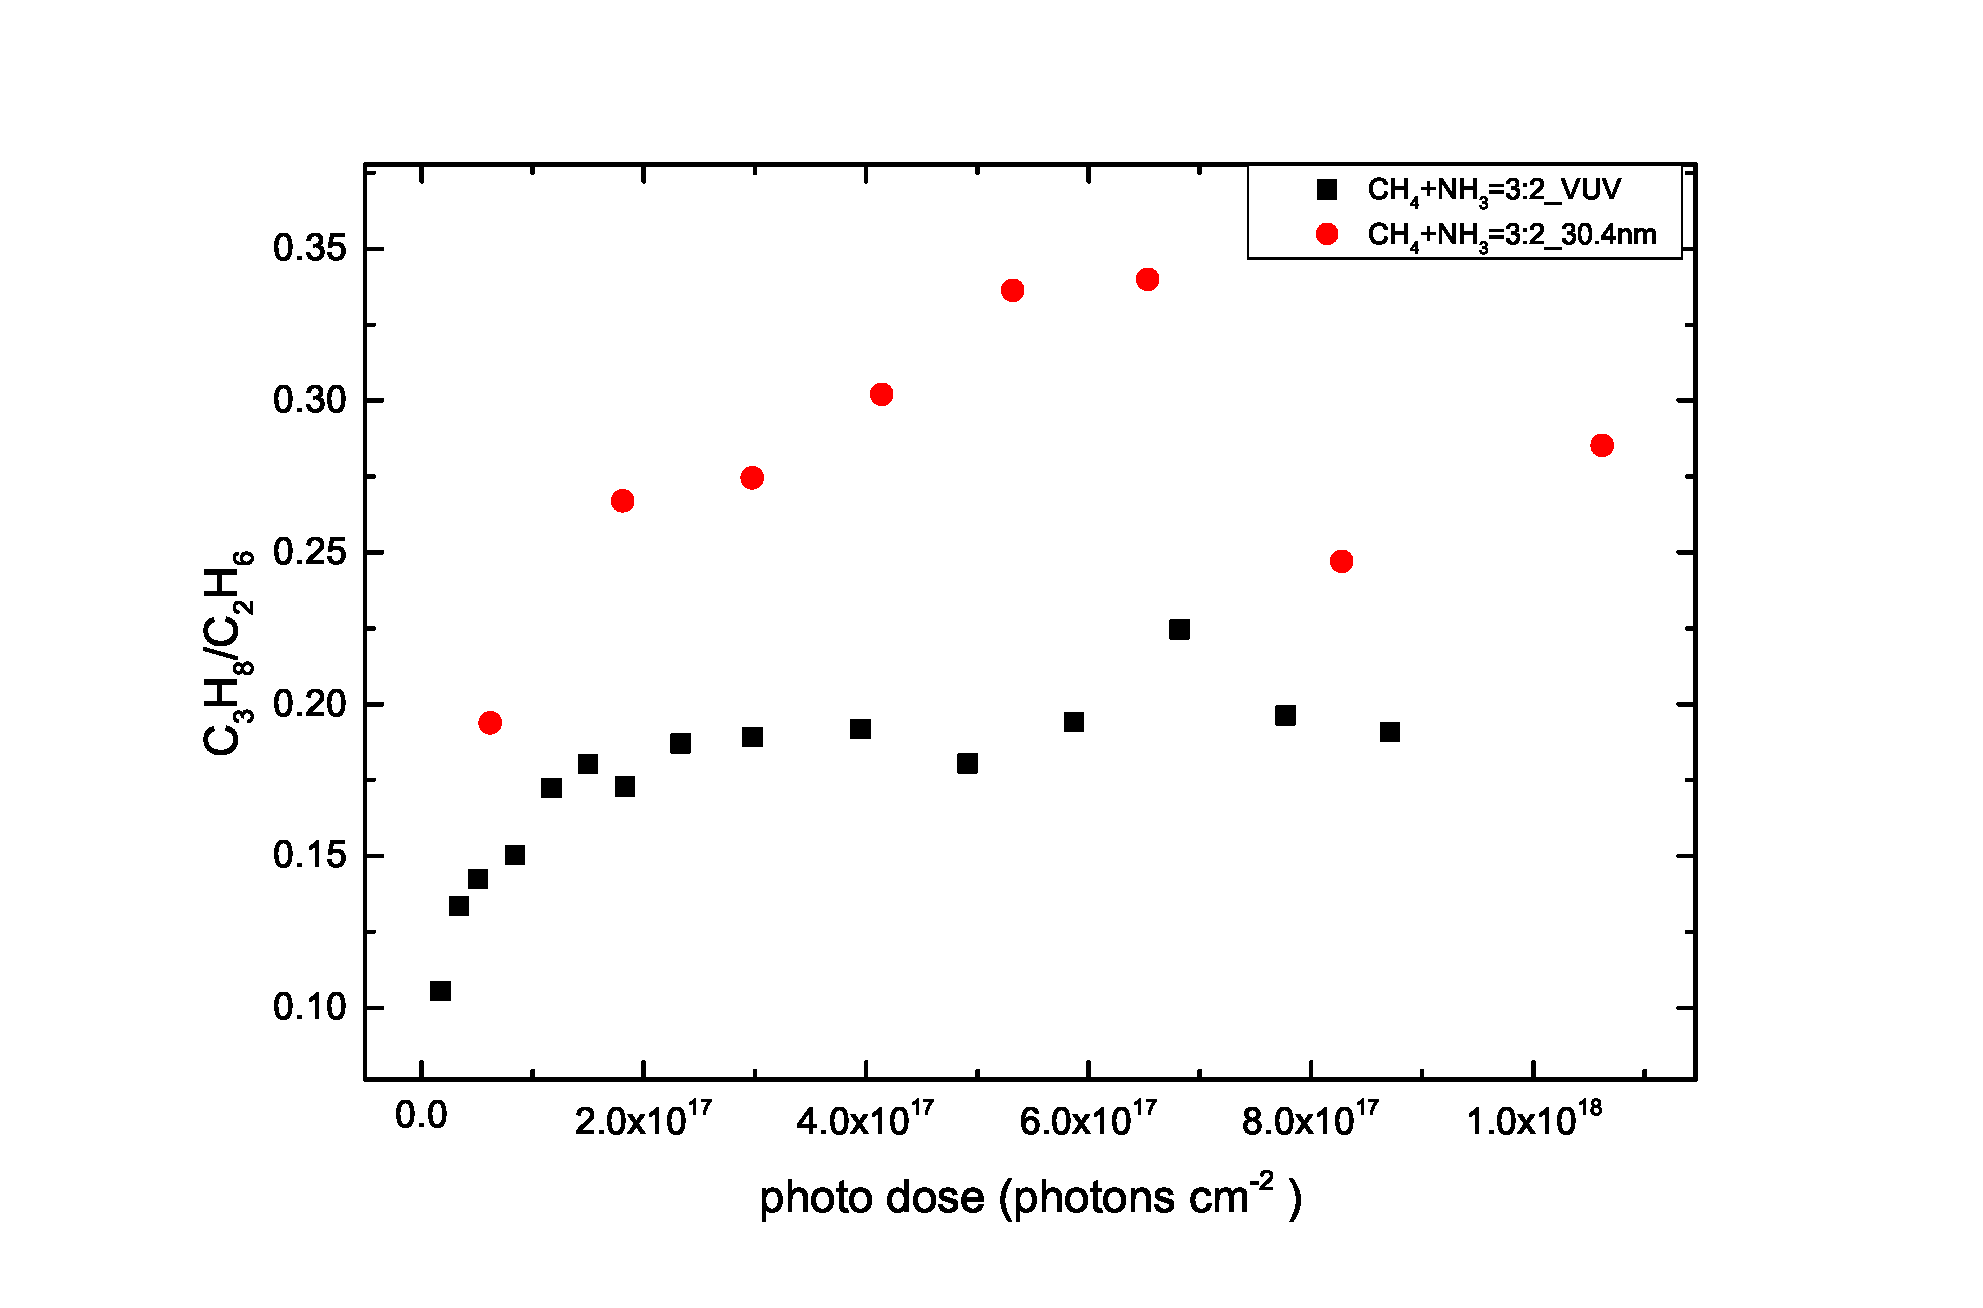
\includegraphics[width=\textwidth]{figures/chapter3/NSRRC_Lab_C3H8_C2H6.eps}
\caption{The column density of C$_3$H$_8$ divided by C$_2$H$_6$ accumulated when different configurations of CH$_4$ + NH$_3$ ice mixtures are irradiated by VUV and EUV photons}
\label{fig:NSRRC_Lab_C3H8_C2H6}
\end{figure}

Figure \ref{fig:NSRRC_Lab_C3H8_C2H6} shows the column densities of C$_2$H$_6$ divided by C$_3$H$_8$ after CH$_4$ + NH$_3$ =3:2 ice mixtures are irradiated by VUV irradiation and He II monochromatic light.

From \ref{fig:NSRRC_Lab_C3H8_C2H6}, we may observe that more C$_3$H$_8$ is produced by 30.4nm photons than by VUV photons. Recall the formation mechanism of C$_3$H$_8$ (equation \ref{eq:C3H82}), CH$_2$ and C$_2$H$_4$ radicals are esccential in producing C$_3$H$_8$. This increase production in C$_3$H$_8$ may be caused by the increase in CH$_2$ radicals during fragmentation of CH$_4$. This result is similar to the findings of Gans et al. (2011)\cite{gans2011photolysis}, the ratio of CH$_2$ radicals increases from 0.3 to 0.48 when photon energy increases from 121.6 nm to 118.2 nm in their pulsed laser experiments.


\begin{figure}
\centering
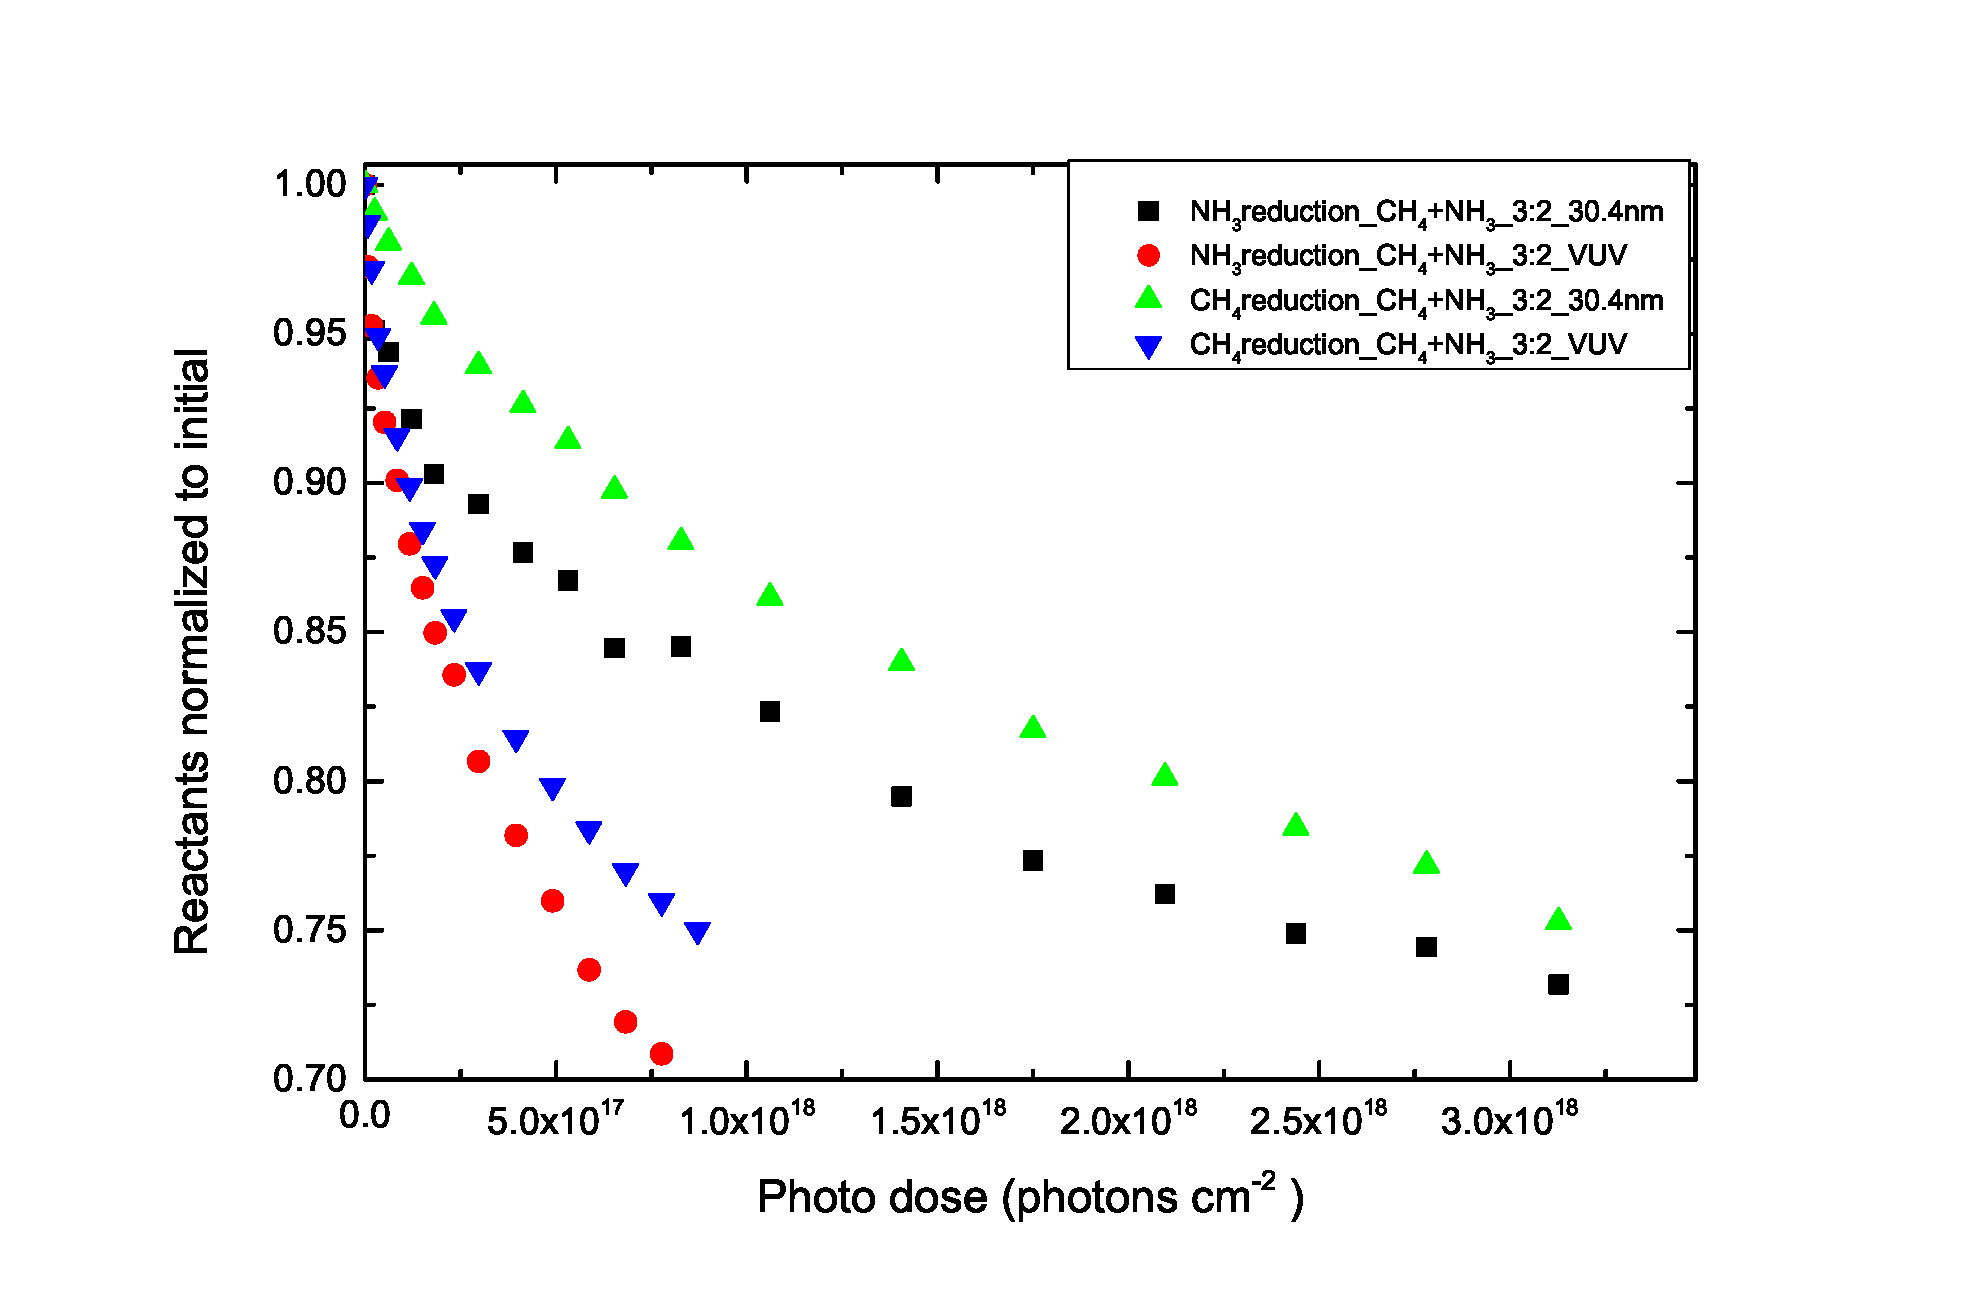
\includegraphics[width=\textwidth]{figures/chapter3/Reactants_normalized_to_initial.eps}
\caption{The normalized reduction of CH$_4$ and NH$_3$ in CH$_4$ + NH$_3$ ice mixtures irradiated by VUV and EUV photons}
\label{fig:normalized_reactants}
\end{figure}


Apart from C$_2$H$_6$ and C$_3$H$_8$, are there any difference in CN$^-$ production? Figure \ref{fig:CN_NSRRC} shows the accumulated column densities of CN$^-$ generated by irradiation of CH$_4$+NH$_3$ ice mixtures by MDHL and 30.4 nm monochromatic light. The fitting results are shown in Table 3.6. The rate constants forming CN$^-$ is 3.06 to 4.13 times larger in CH$_4$+NH$_3$ = 1:5 and 3:2 irradiated by MDHL than irradiated by 30.4 nm monochromatic light respectively. From figure \ref{fig:normalized_reactants}, the destruction cross-section of CH$_4$ and NH$_3$ are reduced by  6.06$\pm$0.07 and 3.19$\pm$0.12 times respectively. The formation rate constants of CN$^-$ is 3.06 to 4.13 times smaller than VUV irradiations (table \ref{CNrate_NSRRC}. Therefore, we may conclude that the reduction in CN$^-$ formation rate by 30.4nm EUV irradiation is mainly due to the decreased NH$_3$ destruction cross-sections.

\begin{figure}
\centering
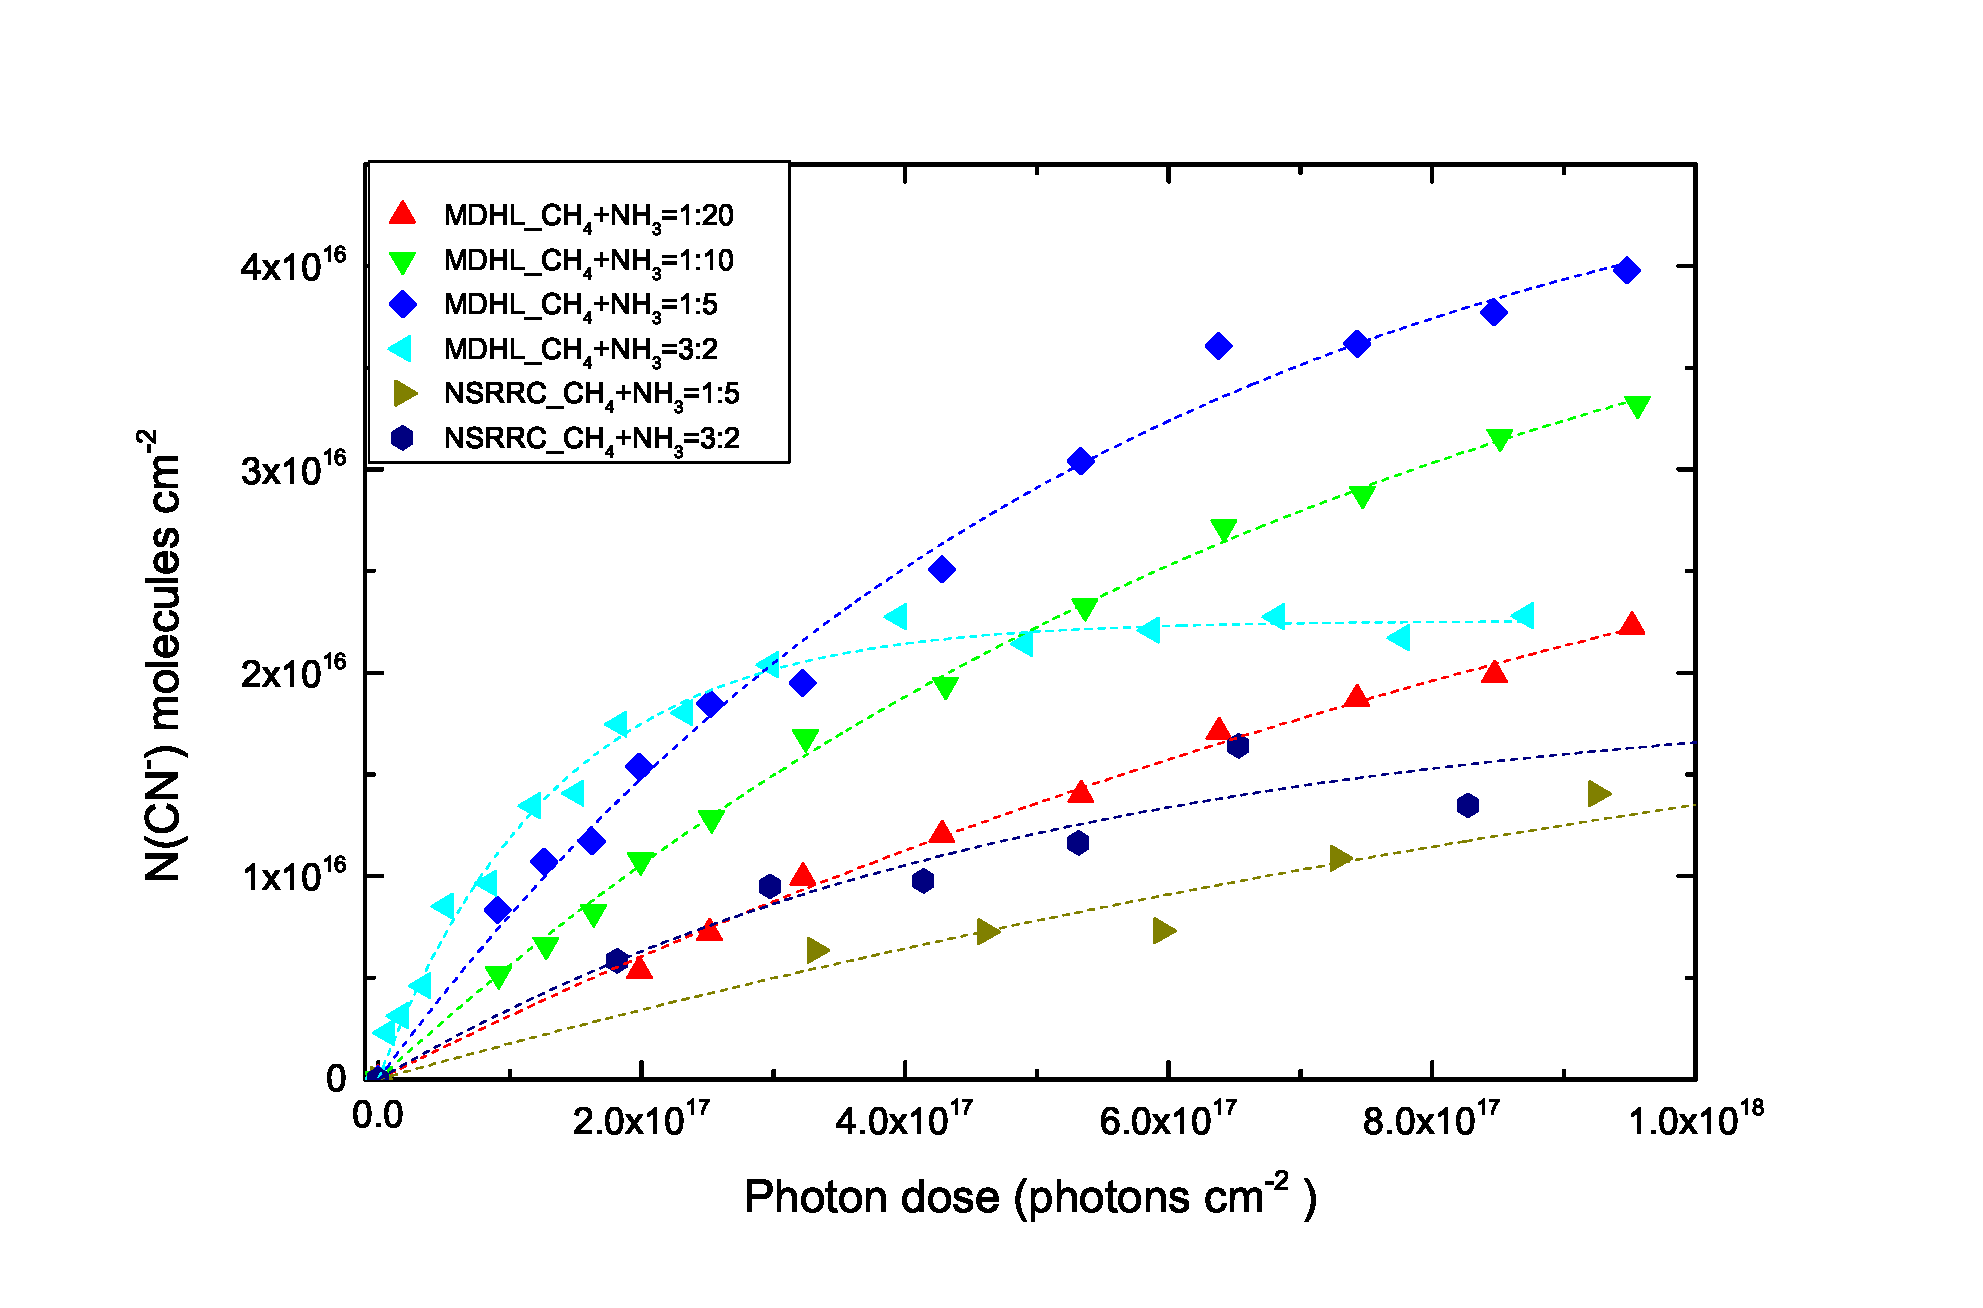
\includegraphics[width=\textwidth]{figures/chapter3/overall_CN_NSRRC.eps}
\caption{The column densities of CN$^-$ generated by irradiation of CH$_4$+NH$_3$ ice mixtures by MDHL and 30.4 nm monochromatic light.}
\label{fig:CN_NSRRC}
\end{figure}

\begin{table}[htbp]
\caption{The fitting results of CN$^-$ by equation \ref{eq:rate7}}
\label{tab:CNrate_NSRRC}
\begin{tabular}{ccccc}
\hline
\hline
Light source & Ratio of CH$_4$+NH$_3$ & A (x10$^{16}$ molecules cm$^{-2}$) & k$_1$ (x10$^{-18}$ photon$^{-1}$) & k$_2$ (photon$^{-1}$)\\
\hline
VUV & 1:5 & 4.61 $\pm$ 0.18 & 1.93 $\pm$ 0.19 & >1 \\
MDHL & 3:2 & 2.24 $\pm$ 0.03 & 8.21 $\pm$ 0.70 & >1 \\
\hline
EUV & 1:5 & 2.89 $\pm$ 1.29 & 0.63 $\pm$ 0.37 & >1 \\
 30.4nm & 3:2 & 2.24 $\pm$ 0.03 & 1.92 $\pm$ 1.99 & >1 \\
\hline
\end{tabular}
Fitting result of figure \ref{fig:CN_NSRRC} with pseudo first order equation [CN$^-$]=$A(1-e^{-kx})$. These fitting results of MDHL experiments are an average of at least 2 experiments with the same circumstances. In the expression, A represents the column density when x, the photon dose, becomes infinitely large and k is the rate constant.\
\end{table}


\section{Residues}
The residues we studied are the accumulated residues onto the substrate. We do not understand are there any interaction between residues and the ice mixtures. However, we may know what is the change of residues when we change the ratio of the CH$_4$+NH$_3$ from CH$_4$ dominating to NH$_3$ dominating.  Figure \ref{fig:residues} is a comparison of CH$_4$+NH$_3$ = 3:2 after VUV experiments, residues accumulated after EUV exposure of CH$_4$ + NH$_3$ = 3:2 ice mixtures and the plasma experiment done by Imanaka et al. (2004)\cite{imanaka2004laboratory}. The residues in ammonia dominated ice mixtures cannot be detected after consecutive experiments. There are no differences between EUV accumulated residues and VUV accumulated residues in CH$_4$+NH$_3$ = 3:2 ice mixtues. The main differences between plasma experiments of N$_2$+CH$_4$ (9:1) done at 2300 Pa. by Imanaka et al. (2004)\cite{imanaka2004laboratory} and our experiments is the peaks located around 2090 cm$^{-1}$.

Why we use different initial reactants, replacing N$_2$ by NH$_3$ but we may get similar residues? The similarities during formation of atomic nitrogens when breaking N$_2$ bonds in nitrogen and NH bonds in ammonia give rise to this result. When photon energy is enough to break both NH bond and N$_2$ bond, similar experimental residues forms. Our results implies that the residues formed on Charon is similar to what we found on Titan, although their formation environments differs from gaseous phase with N$_2$ dominating to solid phase with NH$_3$.


\begin{figure}
\centering
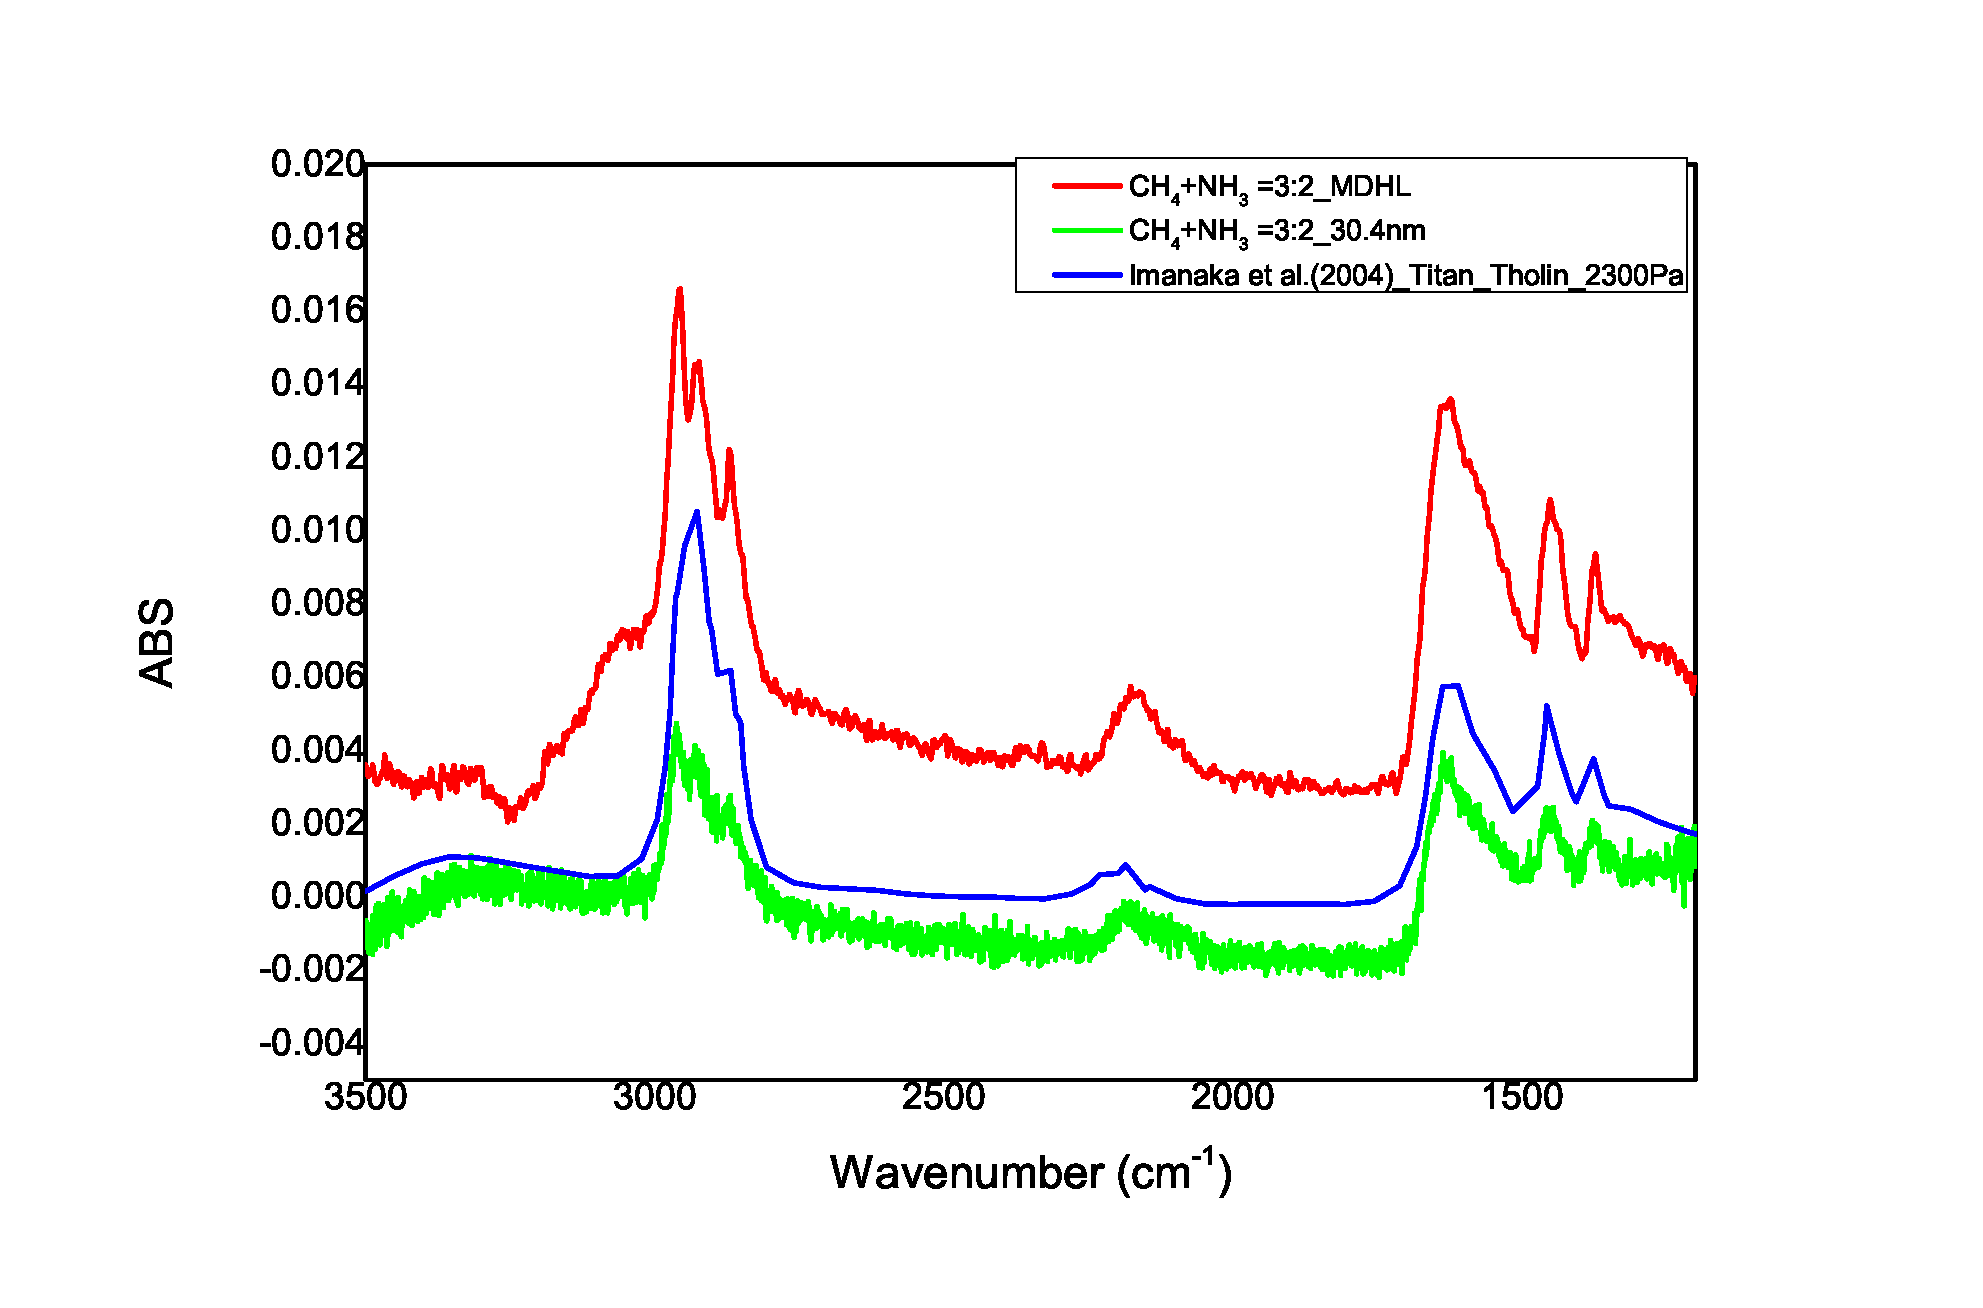
\includegraphics[width=\textwidth]{figures/chapter3/residue.eps}
\caption{The IR spectrum of residues in after CH$_4$+NH$_3$ = 3:2 experiments and the accumulate residues after MDHL experiments and NSRRC experiments.}
\label{fig:residues}
\end{figure}


\section{Conclusion} % should be in chapter 4?

The main product of VUV and EUV irradiated CH$_4$+NH$_3$ ice mixtures are C$_2$H$_6$ and CN$^-$. C$_3$H$_8$ is also produced by C$_2$H$_6$ or C$_2$H$_2$. We did several investigations towards CH$_4$+NH$_3$ ice mixtures. First, by changing ratio of CH$_4$ and NH$_3$ in the ice mixture, CN$^-$ production is more effective in NH$_3$ dominated ice mixtures where C$_2$H$_6$ dominates in CH$_4$ dominated ice mixtures. Second, by changing the photon source to EUV irradiation, the yield of C$_3$H$_8$ increases. The effective formation of C$_3$H$_8$ was not produced by C$_2$H$_6$ but by C$_2$H$_2$ and CH$_4$ because the ratio of C$_3$H$_8$ : C$_2$H$_6$ increases. This suggests that the CH$_2$ or CH fragmentation from CH$_4$ increases when photon energy increases. By studying the production efficiencies, the difference in photo-production yield is mainly caused by the reduction in photo-destruction cross-section in the reactants. Thirdly, by comparison with electron irradiation experiments, electron irradiation has a smaller absorption cross-sections, the percentage of yield is also smaller than VUV irradiated ice mixtures with similar ice thicknesses. Finally, we compared our residues obtained with laboratory produced Taitan tholins, the similar infra-red spectrum shows a similar functional groups in residues. Our result implies that the tholin on Charon should be similar to the tholin formed on Titan.


